\documentclass[11pt]{article}
\usepackage{UF_FRED_paper_style}

\usepackage{lipsum}  %% Package to create dummy text (comment or erase before start)
\usepackage{enumitem}
\usepackage{tikz}
\usepackage{mathrsfs}
\usepackage{threeparttable}
\usepackage{amsmath}
\usepackage{booktabs}
\usepackage{caption}
\usepackage{graphicx}
\usepackage{enumitem}
\usepackage[T1]{fontenc}
\usepackage[utf8]{inputenc}
%% ===============================================
%% Setting the line spacing (3 options: only pick one)
% \doublespacing
% \singlespacing
\onehalfspacing
%% ===============================================

%\setlength{\droptitle}{-5em} %% Don't touch

%% ===============================================
% Set up paper stats 
%% ===============================================
\usepackage{datatool}

\DTLloaddb[keys={title,value}]{stats}{paper_stats.csv}
\newcommand{\getstat}[1]{%
  \DTLfetch{stats}{title}{#1}{value}\unskip
}

% footnotelinepenalty, make sure on same page
\interfootnotelinepenalty=10000

% %%%%%%%%%%%%%%%%%%%%%%%%%%%%%%%%%%%%%%%%%%%%%%%%%%%%%%%%%%
% SET THE TITLE
% %%%%%%%%%%%%%%%%%%%%%%%%%%%%%%%%%%%%%%%%%%%%%%%%%%%%%%%%%%

% TITLE:
\title{\textbf{Heterogeneity in Sectoral Production and the Macro Effect of Sectoral Shocks}
\thanks{I am deeply grateful to Aaron Amburgey, Vivek Bhattacharya, Lawrence Christiano, Martin Eichenbaum, Joseph Ferrie, Gaston Illanes, Benjamin Jones, Diego Känzig, José Luis Lara, Giorgio Primiceri, Ramya Raghanavan, Matthew Rognlie, and Alireza Tahbaz-Salehi for their feedback over the course of this project.}}

% AUTHORS:
\author{Jacob Toner Gosselin\\% Name author
    \href{mailto:jacob.gosselin@u.northwestern.edu}{Northwestern University} %% Email author 1 
    }
    
% DATE:
\date{\today}

% %%%%%%%%%%%%%%%%%%%%%%%%%%%%%%%%%%%%%%%%%%%%%%%%%%%%%%%%%%
% %%%%%%%%%%%%%%%%%%%%%%%%%%%%%%%%%%%%%%%%%%%%%%%%%%%%%%%%%%
\begin{document}
\captionsetup{justification=centering, singlelinecheck=false}
% %%%%%%%%%%%%%%%%%%%%%%%%%%%%%%%%%%%%%%%%%%%%%%%%%%%%%%%%%%
% %%%%%%%%%%%%%%%%%%%%%%%%%%%%%%%%%%%%%%%%%%%%%%%%%%%%%%%%%%
% ABSTRACT
% %%%%%%%%%%%%%%%%%%%%%%%%%%%%%%%%%%%%%%%%%%%%%%%%%%%%%%%%%%
% %%%%%%%%%%%%%%%%%%%%%%%%%%%%%%%%%%%%%%%%%%%%%%%%%%%%%%%%%%
\vfill
{\setstretch{.8}
\maketitle
% %%%%%%%%%%%%%%%%%%
\begin{abstract}
% CONTENT OF ABS HERE--------------------------------------

The effect of a negative sectoral shock on GDP depends on how important the shocked sector is as a direct and indirect supplier and how easily sectors can substitute inputs. Past estimates of the parameters that determine these qualities in the US have been restrictive: they have not been allowed to vary across industries or across time. This paper uses a novel empirical strategy to relax those restrictions, by exploiting variation in input expenditure share shifts within industries rather than across industries. The resulting estimates exhibit significant sectoral and temporal heterogeneity, and are dynamically correlated with weighted patents. In a calibrated GE model of multi-sector production, this heterogeneity (1) raises[lowers] the GDP effect of negative shocks to sectors whose customers are less[more] able to substitute inputs (e.g. the GDP effect of ``Chemical products'' shocks rises), (2) raises[lowers] the GDP effect of negative sectoral shocks in years where sectors are less[more] able to substitute inputs, and (3) raises[lowers] the GDP effect of negative shocks to sectors as they become more[less] central input suppliers (e.g. between 1997 and 2023 the GDP effect of ``Paper products'' shocks fell and the GDP effect of ``Computer and electronic products'' shocks rose due to changes in their importance as input suppliers). 

% END CONTENT ABS------------------------------------------
\noindent
\textit{\textbf{Keywords: }%
Production networks, Sectoral production, Micro-to-macro propagation} \\ %% <-- Keywords HERE!
\noindent
\textit{\textbf{JEL Classification: }%
D24, E23} %% <-- JEL code HERE!
\end{abstract}
}
\vfill


% %%%%%%%%%%%%%%%%%%%%%%%%%%%%%%%%%%%%%%%%%%%%%%%%%%%%%%%%%%
% %%%%%%%%%%%%%%%%%%%%%%%%%%%%%%%%%%%%%%%%%%%%%%%%%%%%%%%%%%
% BODY OF THE DOCUMENT
% %%%%%%%%%%%%%%%%%%%%%%%%%%%%%%%%%%%%%%%%%%%%%%%%%%%%%%%%%%
% %%%%%%%%%%%%%%%%%%%%%%%%%%%%%%%%%%%%%%%%%%%%%%%%%%%%%%%%%%

\section*{Introduction}

Consider a shock which significantly cuts the output of a US industry: a tornado hits Gary, IN, where the bulk of US steel is produced, or a cyber-attack disrupts internet access in San Francisco, a hub of domestic data processing.\footnote{I use ``industry'' and ``sector'' interchangeably throughout the paper.} What would happen to GDP? A natural answer this classic question of micro-to-macro propagation is to use Hulten's theorem: In an efficient economy, the first-order effect on GDP of a shock which cuts output in sector $i$ by $X$\% is $X \times D_i$\%, where $D_i=$ sector $i$'s revenue divided by GDP. But the utility of Hulten's theorem in this context depends on how accurate the first-order approximation is. If shocks are moderate, and propagation is non-linear, the first-order approximation Hulten's theorem provides can be quite misleading. 

The full macro effect of sectoral shocks depends on (1) how important the shocked sector is as a direct and indirect supplier of other sectors, and (2) how easily sectors can substitute inputs. In models of multi-sector production these features depend on two sets of parameters: the elasticity of substitution across intermediate inputs, and industry-input share parameters. Despite their importance, estimates of these parameters for US industries have been restrictive. Existing estimates assume (A) the elasticity of substitution is common across sectors, and (B) both the elasticity of substitution and industry-input share parameters are constant across time.\footnote{Recent work by \citet{comepoirierReallocationHeterogeneousElasticities2023} allows elasticities to vary across 14 major US industries. I discuss how my work differs in detail below.} 

In this paper I estimate time-varying and industry-varying elasticities of substitution, and year-over-year changes in industry-input share parameters, for 66 US industries between 1997-2023. My results reveal meaningful sectoral and temporal heterogeneity in both sets of parameters. I demonstrate that this heterogeneity is quantitatively important, changing predictions of micro-to-macro propagation in a standard GE model of multi-sector production calibrated to the US economy.

To allow for heterogeneity in my parameters of interest, I model sectoral production as a nested-CES function indexed at the sector-year level. I embed this multi-sector production framework in a static, general equilibrium model. Using the stylized example of a vertical supply chain, I demonstrate how both sectoral and temporal variation in these parameters changes the predicted micro-to-macro propagation of sectoral shocks. 

I estimate these parameters using changes in sector-to-sector expenditure shares constructed from the Bureau of Economic Analysis (BEA) input-output accounts. These changes provide variation at the industry-input-year level, for 66 major US industries (roughly corresponding to 3-digit NAICS). Past work has not fully leveraged this feature of the data, relying on variation \textit{across} industries to estimate all parameters of sectoral production \citep{atalayHowImportantAre2017}. Because I solely focus on parameters related to intermediate inputs, I am able to exclusively use variation in expenditure share shifts \textit{within} industries and across inputs. Due to well-known properties of CES aggregation, this variation allows me to identify my parameters of interest with more precision and granularity than previously documented. I test the external validity of my estimates by examining their dynamic correlation with sectoral innovation, as measured by weighted patents; the results are reassuring. My estimates indicate that US sectoral production exhibits gross complementarity in all sectors and all years, strengthening past work documenting the same result under stronger assumptions \citep{atalayHowImportantAre2017}. They further indicate that (1) the ability of US industries to substitute inputs varies meaningfully across sectors (elasticities are heterogenous across sectors in all years), (2) the ability of US industries to substitute inputs varies meaningfully across years (elasticities are heterogenous across years in all sectors), and (3) the production functions of US industries evolve over time in ways that alter the relative importance of inputs (share parameters shift year-over-year).

Revisiting my stylized example, I emphasize the economic interpretation of these three empirical results. Result (1) implies the macro effect of sectoral shocks will vary depending on the elasticities of the direct and indirect customers of the shocked sectors. Result (2) implies the macro effect of sectoral shocks will vary depending on the elasticities in the year of the shock. Result (3) implies the macro effect of sectoral shocks will vary depending on the importance of the shocked sectors as input suppliers in the year of the shock. I ground these implications, and confirm their real-world relevance, with two sets of quantitative exercises.\footnote{``Macro effect'' refers to the sectoral shock's effect on GDP. I use this shorthand throughout the paper.}  

Calibrating my model to the US multi-sector economy, I first examine how my elasticity results alter predictions of micro-to-macro propagation. I simulate severe shocks to individual sectors and compare results using sector-specific elasticity estimates versus imposing the corresponding mean uniformly. I find that sectoral heterogeneity raises[lowers] the macro effect of severe negative shocks to sectors whose customers are less[more] able to substitute inputs. In particular, ignoring sectoral heterogeneity underestimates the macro effect of ``Chemical products'' shocks by 10\%. I then simulate realistic sectoral shocks and compare results using using a “high” elasticity calibration, where each sectors elasticity is set to the 75th percentile of its distribution across years, and a “low” elasticity calibration, where each sector's elasticity is set to the 25th percentile of its distribution across years. I find that the temporal heterogeneity represented in this exercise has similar quantitative importance to relaxing the assumption of Cobb-Douglas production across sectors (i.e. assuming Hulten's theorem is precise).

I then examine how my share parameter results alter predictions. I generate a counterfactual set of share parameters corresponding to my estimates of share parameter shifts between 1997 and 2023. I compare the changes in sectoral output these counterfactuals imply in my model to observed sectoral output growth, and note a close correspondence. I find that some sectors have become more important in the production of other goods (e.g. ``Computer and electronic products''), while others have become less important (e.g. ``Paper products''), shifting the macro effect of severe shocks to those sectors correspondingly. I project linear trends in share parameters to examine the macro effect of severe sectoral shocks in the future.

Following a review of the literature, the paper will be divided into three sections. Section \ref{sec:theory} presents my theoretical framework: I describe my model, examine the theoretical relevance of my parameters of interest, and derive the reduced form I use to estimate my parameters. Section \ref{sec:empirical} contains my empirical work: I review my data sources and variable construction, formalize my empirical specification, and present my empirical results. Section \ref{sec:discussion} covers my quantitative results: I review the economic implications of my empirical estimates, and ground these implications with a series of quantitative exercises.

\subsection*{Related literature}

My paper contributes to the modern literature on production networks. Much of the work in this literature adapts the framework of \citet{acemogluNetworkOriginsAggregate2012}, which imposes Cobb-Douglas sectoral production. I relax this assumption, modeling production as a more general nested-CES function with empirically estimated parameters.

\citet{baqaeeMacroeconomicImpactMicroeconomic2019} also use nested-CES production in their work demonstrating how non-linear propagation can compromise the predictive power of Hulten's theorem and increase the macro effect of negative sectoral shocks. I extend their work by explicitly permitting and estimating time-varying and industry-varying production parameters, and quantifying the relevance of this heterogeneity to micro-to-macro propagation in the US economy.

\citet{atalayHowImportantAre2017} provides the most popular estimates of US sectoral production parameters, using changes in industry-input expenditure shares instrumented with military spending shocks to estimate (1) the outer-nest elasticity of substitution between value-added production and intermediate inputs, and (2) the inner-nest elasticity of substitution across intermediate inputs. He imposes both to be common across sectors and across years. \citet{miranda-pintoFlexibilityFrictionsMultisector2022} use the same instrument regression, but permit the outer-nest elasticity of substitution between value-added production and intermediate inputs to vary by sector.\footnote{They also permit the inner-nest elasticity to vary by sector in their regressions, but do not report results, and assume that elasticity is uniform across sectors in their model.} Since the military spending shock instruments vary at the industry-year level, the elasticity estimates in both papers rely on variation across industry-years.

I also use changes in sector-to-sector expenditure shares to pin down my estimates. However, by focusing on the inner-nest parameters governing intermediate inputs, I do not need to rely on an instrument to avoid endogeneity, and can instead use variation \textit{within} industry-years and across inputs to identify my parameters.\footnote{A more in-depth description of my empirical approach as compared to \citet{atalayHowImportantAre2017} and \citet{miranda-pintoFlexibilityFrictionsMultisector2022} can be found in Appendix \ref{ap:atalay}.} This type of variation is quite powerful when combined with the assumptions of CES aggregation, namely symmetry in substitution across input pairs and indirect explicit additivity \citep{matsuyamaNonCESAggregatorsGuided2023}. It allows me to produce precise industry-varying and year-varying estimates of the inner-nest elasticity of substitution across intermediate inputs, and gives a structural interpretation to the residualized variation in expenditure shares: changes in industry-input share parameters. This measure has not been previously estimated in the literature, to my knowledge; its closest parallel is in the demand literature, where the time-varying residuals of a CES demand system are often treated as consumer taste shock \citep{reddingMeasuringAggregatePrice2020}. It allows me to validate my empirical strategy externally, by showing that my residuals are dynamically correlated with other measures of innovation, namely weighted patents as measured in \cite{koganTechnologicalInnovationResource2017}. 

\citet{comepoirierReallocationHeterogeneousElasticities2023} estimate sector-varying elasticities for 14 US industries between 1997 and 2018, using full-information Bayesian estimation. I estimate sector-varying elasticities for a more disaggregated set of 66 US industries, which increases the capacity for sectoral heterogeneity to alter micro-to-macro propagation. I also estimate year-varying elasticities, and document meaningful temporal heterogeneity which is quantitatively significant for the macro effect of sectoral shocks. Finally, I don't impose constant share parameters, and instead document meaningful year-over-year share parameter shifts that correspond with measures in sectoral innovation (patents) and are also quantitatively significant for the macro effect of sectoral shocks.

% --------------------
\section{Theoretical framework}
\label{sec:theory}
% --------------------

In this section I outline my baseline mode and highlight the exogenous parameters of interest in my paper: the elasticity of substitution across intermediate inputs and industry-input share parameters. I ground their economic interpretation using the stylized example of a vertical supply chain. I also derive the reduced form I use for my empirical estimates of these parameters of interest. 

\subsection{Baseline Model}

Consider a static economy with $N$ sectors at time $t$. For expositional simplicity, I suppress $t$ subscripts in the following lines. All variables should be understood as time-varying, except when specified otherwise.

A representative household supplies one unit of labor inelastically, which is divided into sector-specific labor $\{L_i\}$. The household consumes by maximizing a CES aggregator across sectoral goods, subject to its budget constraint.  
\[
C = \max \left(\sum_i^N \beta_i^{\frac{1}{\nu}} C_i^{\frac{\nu-1}{\nu}}\right)^{\frac{\nu}{\nu-1}} \text{ subject to } \sum_i^N P_i C_i = \sum_i^N W_i L_i
\]

In each sector $i$, there is a representative firm that produces goods $Y_i$ according to the production function\dots

\[ 
\begin{aligned}
Y_i = Z_i \left(\alpha_i^{\frac{1}{\sigma}} L_i^{\frac{\sigma-1}{\sigma}} + (1-\alpha_i)^{\frac{1}{\sigma}} M_i^{\frac{\sigma - 1}{\sigma}} \right)^{\frac{\sigma}{\sigma-1}} \\
M_i = \left(\sum_j^N \omega_{ij}^{\frac{1}{\theta_i}} X_{ij}^{\frac{\theta_i-1}{\theta_i}} \right)^{\frac{\theta_i}{\theta_i-1}}
\end{aligned}
\]

Note that production is nested-CES: the outer nest is a CES aggregator of sector-specific labor $L_i$ and the intermediate input bundle $M_i$, and the inner nest is a CES aggregator of sector-specific goods $X_{ij}$. Assume that\dots

\begin{enumerate}[label=A.\arabic*]
\item Firms are perfectly competitive price-takers.
\item Technology terms $Z_i$, share parameters $\omega_{ij}$, and elasticities $\theta_i$ are exogenous. 
\item Elasticities $\sigma$ and $\nu$ are exogenous and constant. 
\item Share parameters sum to 1 for each sector, i.e. $\sum_j \omega_{ij} = 1$ for all $i$.
\end{enumerate}

Under these assumptions, I formally define the static general equilibrium as wages $W_i$, prices $P_i$, sectoral outputs $Y_i$, and labor $L_i$, such that 

\begin{enumerate}
\item All firms make profit-maximizing input choices $X_{ij}$, $L_i$. 
\item The representative household makes utility-maximizing consumption choices $C_i$.
\item All goods markets clear, i.e. $Y_i = \sum_j^N X_{ij} + C_i$.  
\item All labor markets clear, i.e. $\sum_i^N L_i = 1$.
\end{enumerate}

With my model defined, consider the role of exogenous parameters $\theta_i$, the elasticity of substitution across intermediate inputs, and $\omega_{ij}$, industry-input share parameters. 

The elasticity of substitution across intermediate inputs $\theta_i$ governs the curvature of the intermediate input bundle isoquants, relating changes in input ratios to changes in the marginal rate of technical substitution (MRTS). Informally, this parameter shapes how easily industry $i$ can substitute across intermediate inputs. As $\theta_i$ rises, the isoquants become straight lines, and output can be maintained with a wide range of input ratios (i.e. using exclusively one input). As $\theta_i$ falls, the isoquants become more curved, and output can be maintained only with specific input ratios (i.e. all inputs are ``essential'').

\[\frac{1}{\theta_i} = \frac{\partial \log (\frac{\partial M_i/\partial X_{ij}}{\partial M_i/\partial X_{ik}})}{\partial \log (\frac{X_{ij}}{X_{ik}})} = \frac{\partial \log MRTS^{j,k}_i}{\partial \log \frac{X_{ij}}{X_{ik}}} \text{ for any $j,k$.} \]

Industry-input share parameters $\omega_{ij}$ govern the ratio of marginal products, holding all else fixed. By extension, they govern the ratio of optimal quantities. Informally, these parameter shapes how important specific intermediate inputs are in production, relative to one another: a rise in $\omega_{ij}$ raises the marginal product and the quantity demanded of good $j$, relative to good $k$, for the intermediate input bundle of sector $i$.

\[
\begin{aligned}
\frac{\partial M_i/\partial X_{ij}}{\partial M_i/\partial X_{ik}} = \left(\frac{\omega_{ij} X_{ik}}{\omega_{ik} X_{ij}}\right)^{\frac{1}{\theta_i}} \text{ for any $i,j,k$.} \\
\frac{X^*_{ij}}{X^*_{ik}} = \frac{\omega_{ij}}{\omega_{ik}} \left(\frac{P_k}{P_j}\right)^{\frac{1}{\theta_i}} \text{ for any $i,j,k$.}
\end{aligned}
\]

To better understand the relevance of these parameters to the macro effect of sectoral shocks, and how their variation across industries and across time can meaningfully alter this propagation, consider the stylized example of a vertical supply chain.

\subsection{Stylized example: Vertical Supply Chain}
\label{subsec:stylized_example}

Given the baseline model defined above, impose that production follows a vertical supply chain, as shown in Figure \ref{fig:vertical_chain}. Each sector produces $Y_i$ as a CES aggregator of a sector-specific input $X_{i1}$ and the output of the previous sector $X_{i2} = Y_{i-1}$, with corresponding share parameters $(\omega_{i1}, \omega_{i2})$, elasticity of substitution $\theta_i$, and Hicks neutral technology $Z_i$.  \footnote{Note that we are collapsing the CES production function to a single nest. This is equivalent to assuming output is Leontief in value-added production and the intermediate input bundle, or that inner and outer nest elasticities are equal and the sector-specific input $X_i$ is sector-specific labor $L_i$.} The representative household only consumes the final good $Y_N$ ($\beta_N = 1$ and $\beta_i = 0$ for $i \neq N$). Assume all sector specific inputs are exogenously fixed at a quantity greater than the output of the preceding sector prior to any shocks ($X_{i1} = \bar{X}_{i1} > Y^0_{i-1}$). There are $T$ periods. 

Suppose sector $N/2$ experiences a negative Hicks neutral technology shock of 10\% at time $t \in [0,T]$; i.e. $\log {Z_{N/2,t}} - \log{Z_{N/2,t-1}} = -0.1$.

\begin{figure}[h]
    \centering
    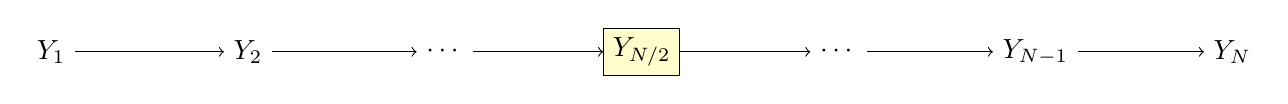
\begin{tikzpicture}[node distance=2.5cm, auto]
        % Nodes
        \node (Y1) {$Y_1$};
        \node (Y2) [right of=Y1] {$Y_2$};
        \node (dots1) [right of=Y2] {$\cdots$};
        \node (YN2) [right of=dots1, fill=yellow!20, draw] {$Y_{N/2}$};
        \node (dots2) [right of=YN2] {$\cdots$};
        \node (YN1) [right of=dots2] {$Y_{N-1}$};
        \node (YN) [right of=YN1] {$Y_N$};
    
        % Arrows
        \draw[->] (Y1) -- (Y2);
        \draw[->] (Y2) -- (dots1);
        \draw[->] (dots1) -- (YN2);
        \draw[->] (YN2) -- (dots2);
        \draw[->] (dots2) -- (YN1);
        \draw[->] (YN1) -- (YN);
    \end{tikzpicture}
    \caption{A vertical supply chain}
    \label{fig:vertical_chain}
\end{figure}

Consider the macro effect of this shock, i.e. its effect on the household consumption bundle $C = Y_N$, in the following scenarios\dots

\begin{enumerate}
    \item All elasticities $\theta_i$ are equal to 1 in all periods. All share parameters are equal to $1/2$ in all periods.
    \item Elasticities $\theta_i$ are equal to 2 for $i \leq N/2$ and 0 for $i > N/2$, in all periods. All share parameters are equal to $1/2$ in all periods.
\end{enumerate}

Scenario 1 corresponds to Cobb-Douglas production, so sectoral propagation is log-linear with a coefficient equal to the corresponding share parameter. The given shock, which reduces the sectoral output of $N/2$ by $-10$\%, will reduce the sectoral output of $N/2+1$ by $-5$\%, $N/2+2$ by $-2.5$\%, and so on. The sectoral output of the final good, and by extension household consumption, will be reduced by $-(10 \times 1/2^{N/2})$\%. 

Scenario 2 corresponds to Leontief production, so sectoral propagation is one-to-one (all inputs are ``essential''). In this case, the given shock will reduce the sectoral output of $N/2+1$ by $-10$\%, the sectoral output of $N/2+2$ by $-10$\%, and so on. Household consumption will be reduced by $-10$\% correspondingly. 

The mean elasticity across industries $\bar{\theta}_i = 1$ in Scenario 2, so imposing and estimating a common elasticity across sectors would imply the same macro effect as Scenario 1. The true macro effect differs in Scenario 2 because the elasticities of the sectors directly and indirectly effected by the shock are lower than the overall average: the shock hits the most ``sensitive'' sectors that are least able to substitute inputs.

Now, consider the macro effect of the same shock in the following alternative scenarios\dots 

\begin{enumerate}
    \item All elasticities $\theta_i$ are equal to 1 in all periods. All share parameters are equal to $1/2$ in all periods.
    \item[2a.] All share parameters are equal to $1/2$ in all periods. At time $t=0$, all elasticities $\theta_{i,0}$ are equal to 0. Over time, firms become better at substituting labor and inputs in production: each period all elasticities increase by $2/T$, so that $\theta_{i,T} = 2$.
    \item[2b.] All elasticities $\theta_i$ are equal to 1 in all periods. At time $t=0$, share parameters $(\omega_{i1,0}, \omega_{i2,0}) = (1,0)$. Over time, the output of the preceding sector becomes more central in production: each period $(\omega_{i1,t}, \omega_{i2,t}) = (\omega_{i1,t-1}-1/T,\omega_{i2,t-1} + 1/T)$, so that $(\omega_{i1,T}, \omega_{i2,T}) = (0,1)$.
\end{enumerate}

The macro effect of the shock in Scenario 1 will again be $-(10 \times (1/2)^{N/2})$\%. In Scenario 2a, the macro effect depends on the period $t$: at $t=0$, the macro effect of the shock is $-10$\%, but at $t=T$, it is $-X$\%, where $X < 10 \times (1/2)^{N/2}$; .\footnote{A formal derivation of this result can be found in Appendix \ref{ap:stylized_example}.} The mean elasticity across time $\bar{\theta}_t = 1$ in Scenario 2a, so imposing and estimating a constant elasticity would imply the same macro effect as Scenario 1. The true macro effect falls gradually between $t = 0$ and $t = T$ as sectors become better at substituting across inputs and therefore less ``sensitive''.

In Scenario 2b, the macro effect also depends on the period $t$. At $t=0$, the macro effect of the shock is $0$\%, but at $t = T$ it is $-10$\%. The mean share parameters across time are $(1/2,1/2)$, so imposing and estimating constant share parameters would imply the same macro effect as Scenario 1. The true macro effect rises gradually between $t=0$ and $t=T$ as the output of the preceding sector becomes more central in each firms' production.

While these examples are stylized, the results are general. Ignoring sectoral heterogeneity in elasticities, temporal heterogeneity in elasticities, or temporal heterogeneity in share parameters, can lead to significant errors in the predicted macro effect of sectoral shocks.\footnote{Generalizations of these results can be seen in \citet{baqaeeMacroeconomicImpactMicroeconomic2019}.} With that in mind, I now turn to the reduced form I use to estimate these parameters, permitting such heterogeneity.

\subsection{Deriving reduced form}

Define $a_{ij}$ as expenditure by industry $i$ on the output of industry $j$ as a share of industry $i$'s total expenditure on intermediate inputs. Define $Q_i$ as the unit cost of industry $i$'s  intermediate input bundle. Via cost-minimization, we can derive the following relation\dots

\[ a_{ij} = Q_i^{\theta_i - 1} P_j^{1 - \theta_i} \omega_{ij} \text{, where } Q_i := \left(\sum_j \omega_{ij} P_j^{1-\theta_i}\right)^{\frac{1}{1-\theta_i}} \text{ and } a_{ij} := \frac{P_j X_{ij}}{Q_i M_i} \]

Expenditure share $a_{ij}$ is the product of unit cost $Q_i$, price $P_j$, and share parameter $\omega_{ij}$, with the first two terms raised to opposite signed powers of the elasticity of substitution across intermediate inputs $\theta_i$. Log-linearizing this equation, and taking the total derivative of both sides, we recover the following relation\dots 

\[
\partial \log a_{ij} = \partial [(\theta_i - 1) \log Q_{i}] + \partial[(1-\theta_i)\log P_j] + \partial \log \omega_{ij}
\]

Note that the first of these three terms is \textbf{fixed at the industry-level, not the industry-input level.} This relation stems from two properties of CES aggregators: indirect explicit additivity, and identical elasticities of substitution between each pair of goods \citep{matsuyamaNonCESAggregatorsGuided2023}. The former ensures that relative demand for any two goods is independent of the price of a third good; the latter ensures that the elasticity parameter governing that relative demand is common across all pairs. The equation above is normalizing expenditure shifts to be relative to the industry-specific intermediate input bundle $M_i$: variation in these relative demand shifts is log-linear in input price, with a residual corresponding to a ``preference shock'' driven by changes in share parameters. Thus, if we assume $\partial \theta_i = 0$, within an industry log changes in industry-input expenditure shares is linear with respect to log changes in input price. The corresponding coefficient is $1-\theta_i$ and the corresponding intercept is $C_i = (\theta_i - 1) \partial(\log Q_{i})$; any residual is equal to log changes in share parameters $\partial \log \omega_{ij}$.

The log-changes in expenditure share I observe are annual, so I rewrite the above equations in terms of first differences over time ($\Delta x_t = x_t - x_{t-1}$). The elasticity of substitution can only be identified at the frequency of the data, so I define $\theta_{it}^1$ as the elasticity governing substitution in response to relative price changes between year $t-1$ and year $t$.\footnote{This is equivalent to assuming constant industry-level elasticities over the course of each year.} We finally recover the relation \dots

\begin{equation}
\label{eq:reduced_form}
\Delta \log a_{ijt} = (\theta^1_{i,t} - 1) \Delta \log Q_{it} + (1-\theta^{1}_{i,t}) \Delta \log P_{jt} + \Delta \log \omega_{ijt}
\end{equation}

This is the reduced form I estimate below. In conclusion, note that by focusing on inner-nest parameters $\theta_i$ and $\omega_{ij}$, we can fully exploit the variation offered by expenditure-shares: each industry has $N$ first order conditions relating $N$ expenditure shares to our parameters of interest. In practice this will mean we can isolate within-industry $ijt$ variation and absorb variation driven by $\Delta \log Q_{it}$. This would not be possible if the goal was to additionally estimate outer-nest parameters like $\sigma$ using expenditure share data, as in \citet{atalayHowImportantAre2017}; a deeper discussion of this point can be seen in Appendix \ref{ap:atalay}. 

% --------------------
\section{Empirical Results}
\label{sec:empirical}
% --------------------

In this section I describe my data construction, formalize my empirical specification corresponding to the reduced form derived above, and present my empirical results.

\subsection{Data construction}

To estimate equation \ref{eq:reduced_form}, I need measurements of changes in industry-input expenditure shares $a_{ij} = \frac{P_j X_{ij}}{Q_i M_i}$ and changes in prices $P_j$. I construct these measurements using data from the BEA Input-Output Accounts and GDP by Industry series.\footnote{All BEA data is pulled from their public API.} 

From the Input-Output Accounts I use the ``Domestic Supply of Commodities by Industry - Summary'' and ``Use of Commodities by Industry - Summary'' tables. These tables provide the supply and use of commodities, in \$, by industries at the BEA summary-level (roughly equivalent to 3-digit NAICS classification), from 1997-2023. I subset the data to only include the 66 non-government summary-level industries.

I normalize the domestic supply of commodities by industry by total commodity output. For each year, I generate a industry-commodity matrix of commodity use, $U_t = \{u_{ict}\} = P_{ct} X_{ict}$, and a commodity-industry matrix of commodity supply, $S_t = \{s_{cjt}\} = \frac{P_{ct} Y_{cjt}}{P_{ct} Y_{ct}}$. I multiply these matrices; the resulting matrix is $\{\text{exp}_{ijt}\}$, where\dots 

\[
\text{exp}_{ijt} = \sum_c \text{u}_{ict} \times s_{cjt} \approx P_{jt} X_{ijt}
\]

In words, I sum the product of (1) spending on commodity $c$ by industry $i$ and (2) the percent of commodity $c$ that is produced by industry $j$, across commodities. The result is a measure of expenditure by industry $i$ on industry $j$. Finally, I normalize this expenditure measure by its row-sum; this normalization gives me expenditure by industry $i$ on industry $j$ as a share of its spending on all intermediate inputs, i.e. $a_{ijt}$.

From the GDP by Industry series, I use the Gross Output tables. These tables provide a ``Chain-Type Price Index for Gross Output'' measure by industry at the summary-level, which is prepared by combining the price indices of the commodities that the industry produces in a Fisher index-number formula. This is an exact measure of $\Delta \log P_{jt}$, presuming industry price is a stable flexible function of commodity prices \citep{diewertExactSuperlativeIndex1976}.\footnote{While I allow the way industries produce goods to evolves over time, I assume the goods they produce do not.}

To assess the external validity of my empirical strategy, I use the weighted patent dataset constructed by \cite{koganTechnologicalInnovationResource2017}, updated through 2023 (henceforth KPSS). KPSS provides patents from 1926-2023, with the Center for Research in Security Prices (CRSP) stock level identifier (permno). KPSS provides citation weights and economic value weights for each patent. 

I use the permno to merge KPSS with the CRSP/Compustat Merged database, where I can recover the NAICS code corresponding to the patent. To match the patent to a BEA summary-level sector, I create a six-digit NAICS to BEA crosswalk. I do this by using the BEA Industry and NAICS Concordance table, which lists associated NAICS codes for each BEA summary-level industry. This concordance table lists codes associated with each summary-level industry at the 2017 NAICS 3-6 digit level. I map this to 6-digit 2022 NAICS codes, as Compustat updates and backfills their NAICS codes \href{https://wrds-www.wharton.upenn.edu/pages/support/support-articles/compustat/general/naics-compustat/#detail}{regularly}. I then use the 6-digit 2022 NAICS code to match each patent to a BEA summary-level industry, and then aggregate total patent counts and citation/value weights by industry-year. The resulting dataset encompasses 2.7 million patents.

Finally, from the Integrated Industry-Level Production Account (KLEMS) (constructed by the BLS and available on their website), I use the Industry TFP tables, which provide a measure of TFP by industry at the summary-level. I use this measure to generate realistic industry-level TFP shocks.

\subsection{Empirical Specification}

In Equation \ref{eq:reduced_form} I state the following reduced form derived from my baseline model.

\[
\Delta \log a_{ijt} = (\theta^1_{i,t} - 1) \Delta \log Q_{it} + (1-\theta^{1}_{i,t}) \Delta \log P_{jt} + \Delta \log \omega_{ijt}
\]

Relying on variation at the industry-year ($it$) level to estimate this equation would require observing changes in the price of the intermediate input bundle $Q_{it}$. This is unobservable in the data under my assumptions. The Fisher index-number formula used to construct a proxy for $Q_{it}$ in the BEA data is an exact measure \textbf{assuming the aggregator function is stable in adjacent periods}. This is a well-known restrictive assumption of such price indices in the demand literature \citep{reddingMeasuringAggregatePrice2020}. 

To get around this issue, I absorb $it$ variation, and estimate my reduced form as\dots 

\[
\Delta \log a_{ijt} = \gamma_{it} + \alpha_{0;i;it} \Delta \log P_{jt} + \epsilon_{ijt}
\]

Where $\gamma_{it}$ represent industry-year fixed effects, and $\alpha$ represent the coefficients on price changes. I list three indices for $\alpha$, as I will estimate the parameter at three levels: common, industry-specific, and industry-year-specific. These three levels correspond to relaxing assumptions of common and constant elasticities.

Note that in order to control for industry-year fixed effects, industry-input-year variation is required: I cannot rely on data that bundles intermediate inputs together. This eliminates high-quality firm-level microdata for the US (e.g. The US Census Annual Survey of Manufacturers reports bundled intermediate-input expenditures as ``MATCOST''). It is for this reason that, despite their highly aggregated nature, the sector-level data provided by the BEA is uniquely well-equipped to identify my parameters of interest. 

Under the assumptions of my baseline model, the resulting estimates $\hat{\alpha}$ correspond to $1-\theta^1$, while the resulting residuals $\epsilon_{ijt}$ correspond to $\Delta \log \omega_{ijt}$. The regression with industry-year coefficients $\alpha_{it}$ has an $R^2$ of $0.22$; the residuals can be seen in Figure \ref{fig:reg_resid}.

\subsection{Empirical Results}

I discuss my estimates of elasticities and share parameter shifts in detail, then summarize the main results and note their robustness.

\subsubsection*{Estimates of elasticities}

I recover elasticity estimates as $\hat{\theta}^1 = 1 - \hat{\alpha}$. My results are best summarized by considering increasing levels of granularity. First, I assume elasticity $\theta^1$ is common across sectors and constant across years, as in \citet{atalayHowImportantAre2017}. I report my resulting ``Uniform'' estimate in Table \ref{tab:atalay_comparison}, and compare it with the corresponding estimate using the IV strategy of \citet{atalayHowImportantAre2017} with my updated data. Our estimates are comfortingly in line, but my standard errors are much lower, especially if I cluster them at the industry-year level (which is appropriate given the industry-year variation provided by the Atalay instruments). This increased precision permits me to estimate elasticities at more granular levels.

\begin{table}[!h]
    \centering 
    \caption{Uniform elasticity estimate}
    \label{tab:atalay_comparison}
    
\begin{tabular}{l c c c c}
\hline
 & \multicolumn{2}{c}{Robust SE} & \multicolumn{2}{c}{Clustered SE} \\
\cline{2-3} \cline{4-5}
 & Uniform & Atalay IV & Uniform & Atalay IV \\
\hline
Elasticity & $0.35$   & $0.41$   & $0.35$   & $0.41$   \\
           & $(0.01)$ & $(0.29)$ & $(0.02)$ & $(1.40)$ \\
\hline
\end{tabular}

\end{table}

Next, I estimate constant sector-specific elasticities $\hat{\theta}^1_i = 1 - \hat{\alpha}_i$. I plot these estimates in Figure \ref{fig:theta_onlyCode}. The dashed lines represents ``realistic gross complementarity'': elasticity values between 0 and 1. The bands represent the 90\% confidence interval.\footnote{I cluster at the industry-year level, but results are unchanged using White SEs.} All but three of my sector-specific elasticity estimates fall within the realistic gross complementarity region, strengthening the finding of \citet{atalayHowImportantAre2017}: complementarity across inputs seems to be common to production in all industries. That said, my estimates reveal meaningful sectoral heterogeneity. Sector-specific estimates vary, and confidence bands often don't overlap.    

\begin{figure}[!h]
    \centering 
    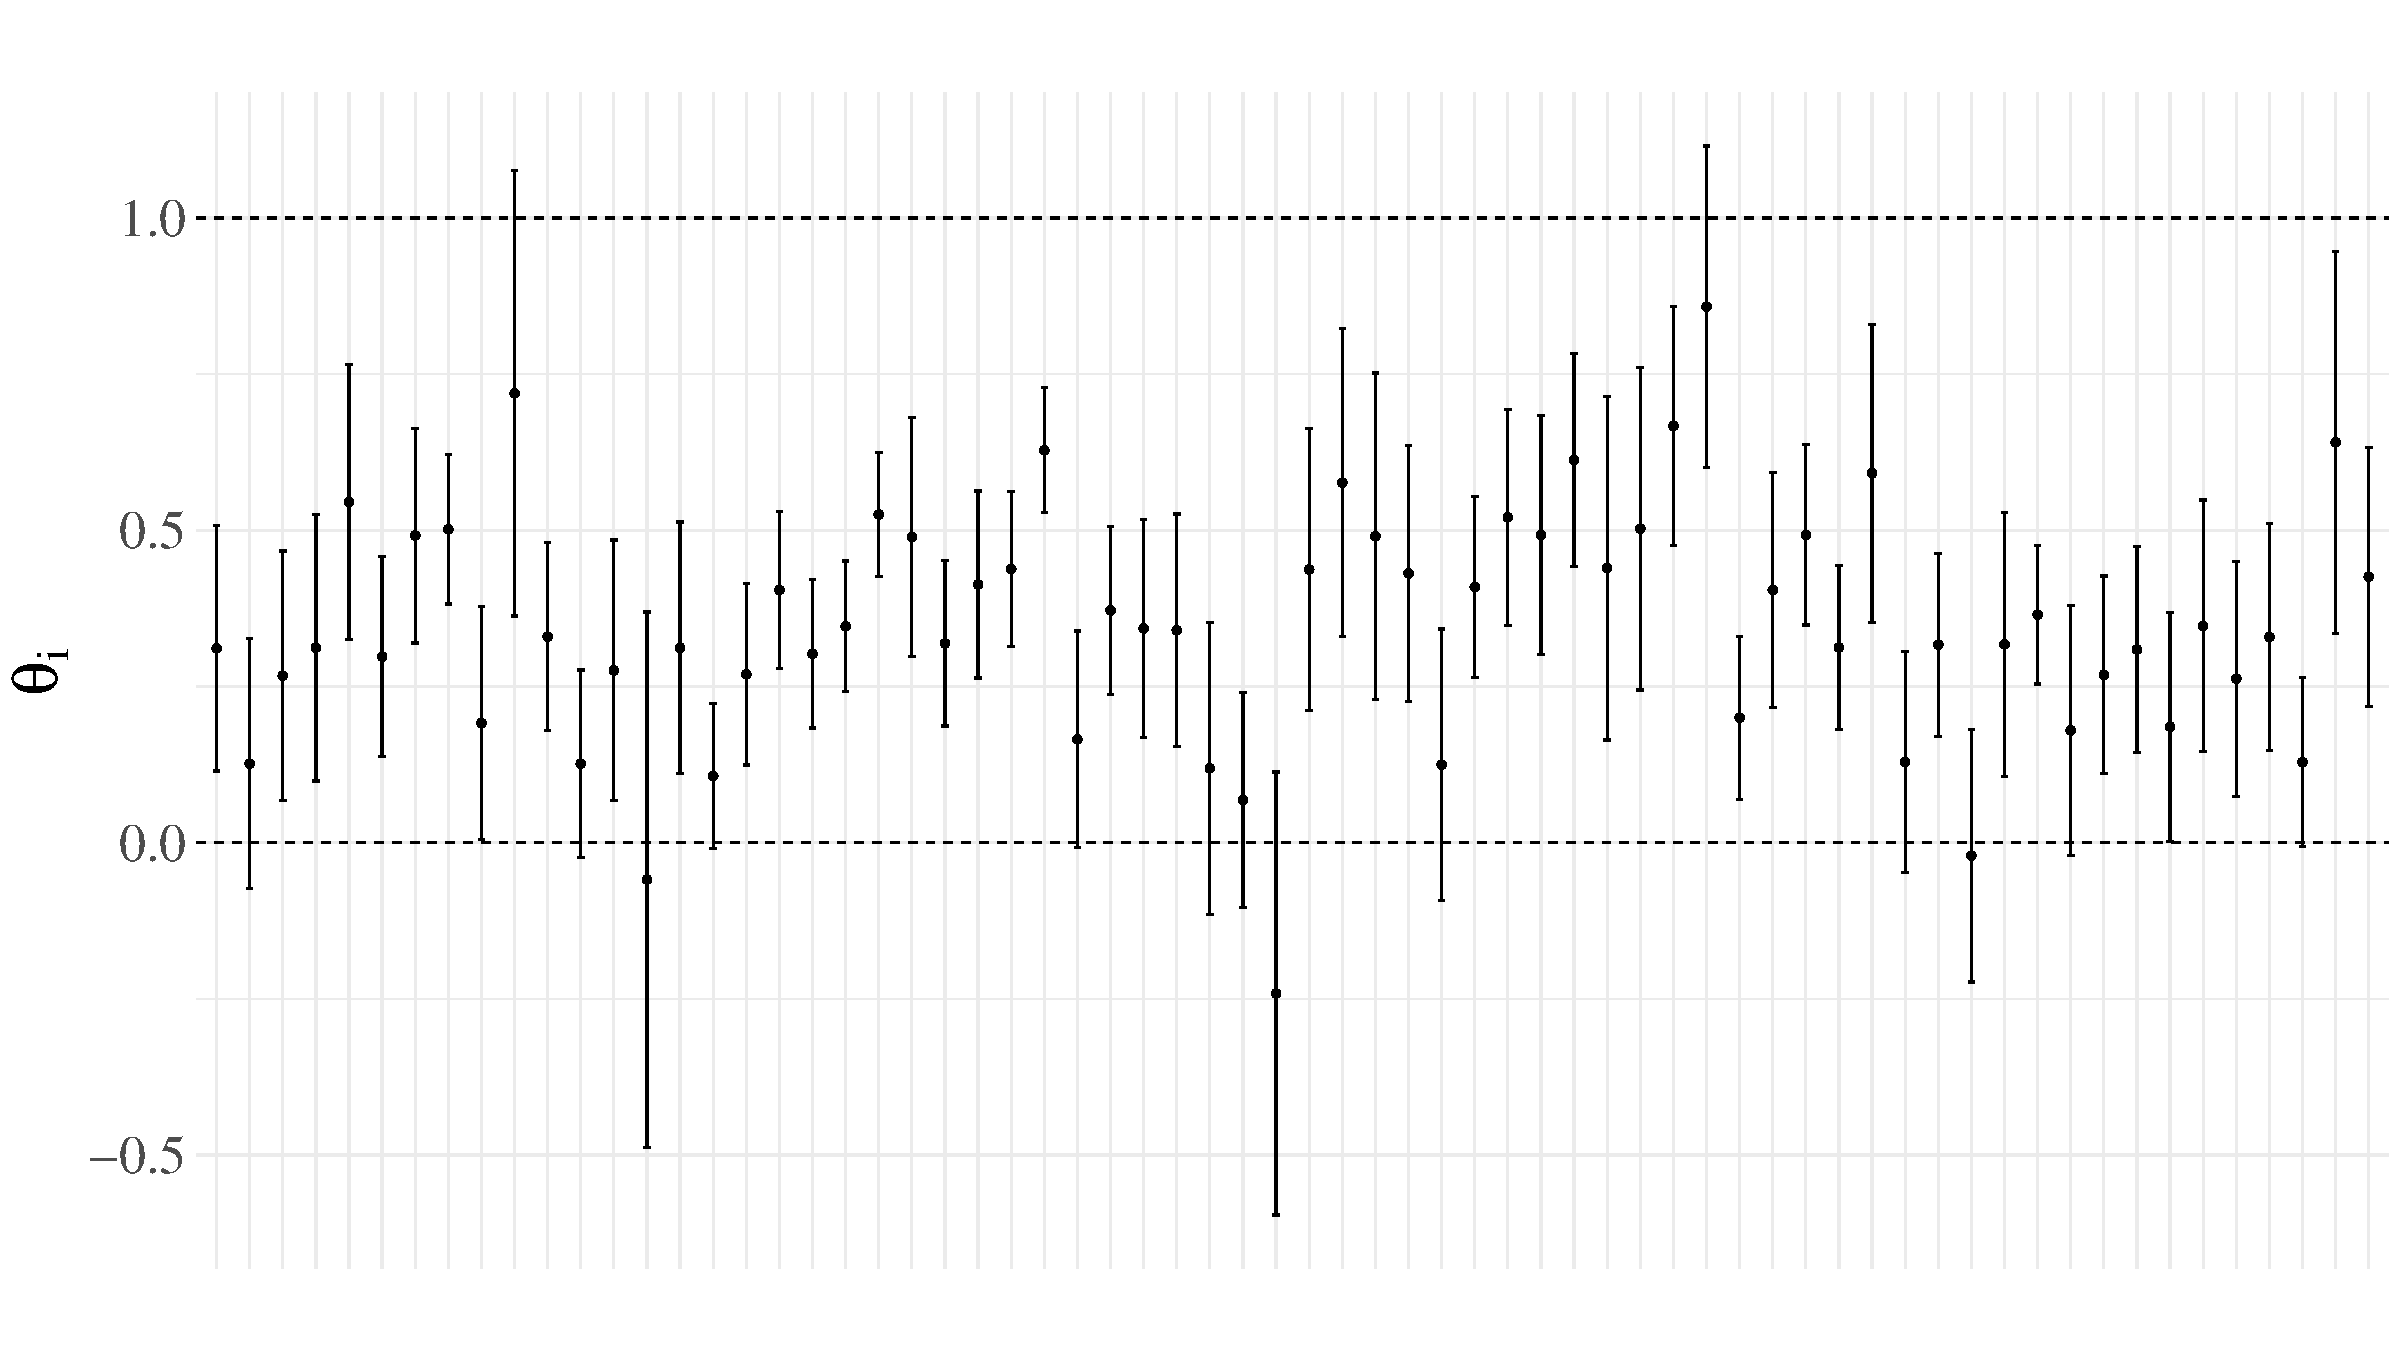
\includegraphics[width=.75\textwidth]{../figures/elasticity_est/elasticity_onlyCode.pdf}
    \caption{Elasticities by industry (constant across years)}
    \label{fig:theta_onlyCode}
\end{figure}

Finally, I estimate industry-year specific elasticities $\hat{\theta}^1_{it} = 1 - \hat{\alpha}_{it}$. I summarize my results in Figure \ref{fig:theta_byYear_byCode}. The points in both plots are $\bar{\theta}^1_t$, the within year and across industry mean, and $\bar{\theta}^1_i$, the within industry and across year mean. The bands and shaded regions represent $\pm$ the corresponding standard deviation of estimates, i.e. across industries within a year in the first panel and across years within an industry in the second. I again include dashed lines representing realistic gross complementarity: the majority of my industry-year estimates fall in this region, further confirming that complementarity across inputs is always and everywhere a feature of sectoral production. 

More importantly, the full extent of sectoral and temporal heterogeneity in the elasticity of substitution is now evident. Within a given year, the standard deviation of elasticity estimates across industries ranges from \getstat{low-sd-year} to \getstat{high-sd-year}, with a median of \getstat{median-sd-year}. Within a given industry, the standard deviation of elasticities across years ranges from \getstat{low-sd-Code} to \getstat{high-sd-Code}, with a median of \getstat{median-sd-Code}. In other words, in all years the elasticity of substitution varies meaningfully across sectors, and in all sectors the elasticity of substitution varies meaningfully across years.

\begin{figure}[!h]
    \centering 
    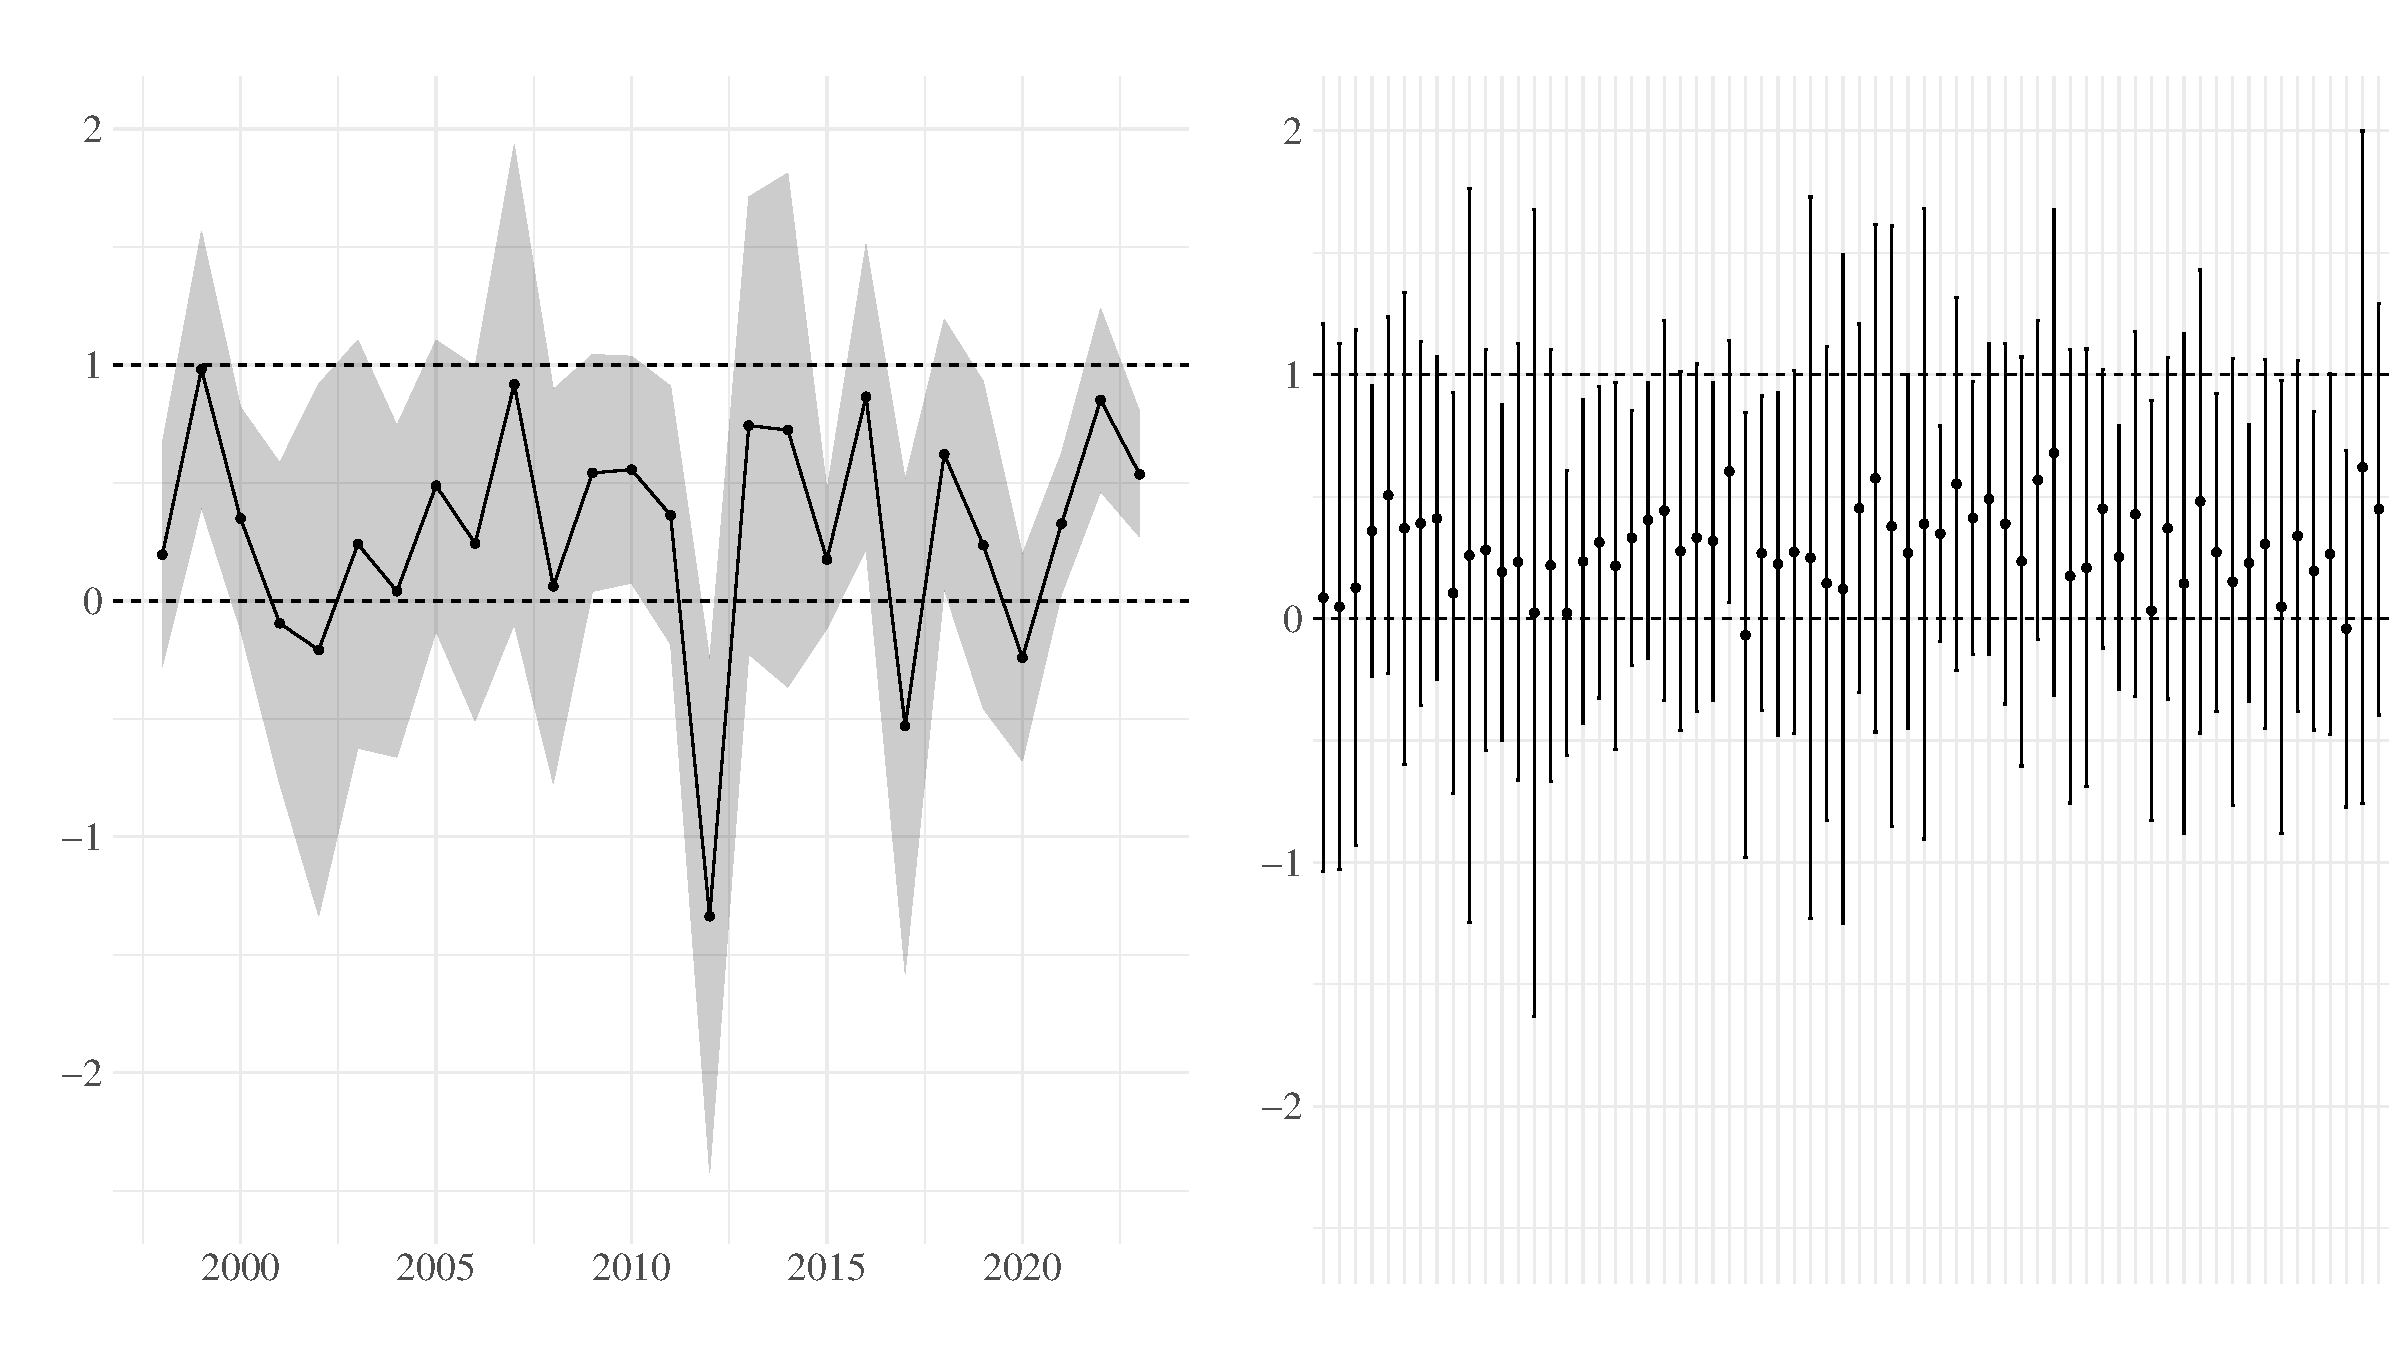
\includegraphics[width=\textwidth]{../figures/elasticity_est/elasticity_byYearAndCode.pdf}
    \caption{Elasticities by industry-year}
    \label{fig:theta_byYear_byCode}
\end{figure}

\subsubsection*{Estimates of share parameter shifts}

As stated above, my residuals $\epsilon_{ijt}$ are an estimate of log-changes in share parameters $\Delta \log \omega_{ijt}$ under the assumptions of my baseline model. As seen in Figure \ref{fig:reg_resid}, there is seemingly a non-trivial number of such changes. This residual variation offers the opportunity to externally validate my results.\footnote{I use residuals $\epsilon_{ijt}$ from the regression with industry-year coefficients $\alpha_{it}$, but results are qualitatively unchanged if I use common coefficient $\alpha_0$ or industry specific coefficients $\alpha_i$.} 

I sum the absolute value of my residuals across inputs for a given industry-year, generating $p_{it}$.

\[
p_{it} = \sum_j |{\epsilon_{ijt}}| 
\]

If I am indeed recovering a reasonable estimate of $\Delta \log \omega_{ijt}$, this absolute sum measures the magnitude of exogenous changes in sectoral production which shifted relative input demand in a given year. It therefore ought to be connected to sectoral innovation. Consider the case of fracking, where a combination of innovations (microseismic fracture mapping, bendable drill housing, etc...) led to the ``shale revolution''. These innovations changed sectoral production of oil and gas extraction in ways that presumably altered the industry's cost-minimizing input mix.\footnote{Comfortingly, my data seems to bear this out: log changes in shale production is positive correlated with the absolute sum of residuals for the ``Oil and gas extraction'' industry.}

With this intuition in mind, I use my sector-level patent measures constructed from KPSS data to estimate the following regressions for $h\in[0,10]$ \dots 

\[
p_{i,t+h} = \beta^h \text{PATENT}_{it} + \gamma_i + \eta_t + \epsilon_{it}
\]

The resulting $\beta^h$ corresponds to the effect of a (weighted) patent in sector $i$ at time $t$ on the absolute sum of residuals $h$ years later, controlling for industry and year fixed effects. 

I plot $\beta^h$ in Figure \ref{fig:patents_citations_resid}, weighting patents by citations. The line shown reflects the estimated effect of a patent with 10,000 citations in a sector on that sector's absolute sum of residuals X-years later. The dark [light] shaded regions correspond to 66\% [90\%] confidence intervals. I see an initially increasing and eventually stable positive effect, significant at $p<.1$ in all periods. I plot $\tilde{\beta}_h$, weighting patents by economic value, in Figure \ref{fig:patents_value_resid}; I see a similar pattern, though the 90\% confidence intervals includes 0 in all but the third period. As discussed in Appendix \ref{ap:historical}, when I extend my sample to include historical data from 1947-1996, I see the same pattern with greater significance: the effect is positive and significant at $p<.1$ from years 1-10, using both citation and value weights.

In sum, the residual recovered from my empirical specification seems to have the economic meaning my assumptions imply; a measure of changes in sector-level production functions. I take the results of my patent regressions as strong suggestive evidence that my baseline assumptions are not meaningfully violated and that my residual variation $\epsilon_{ijt}$ corresponds to share parameter shifts $\Delta \log \omega_{ijt}$, reflecting US sectoral production functions evolving over time in ways that alter relative input demand.

\begin{figure}[!h]
\centering 
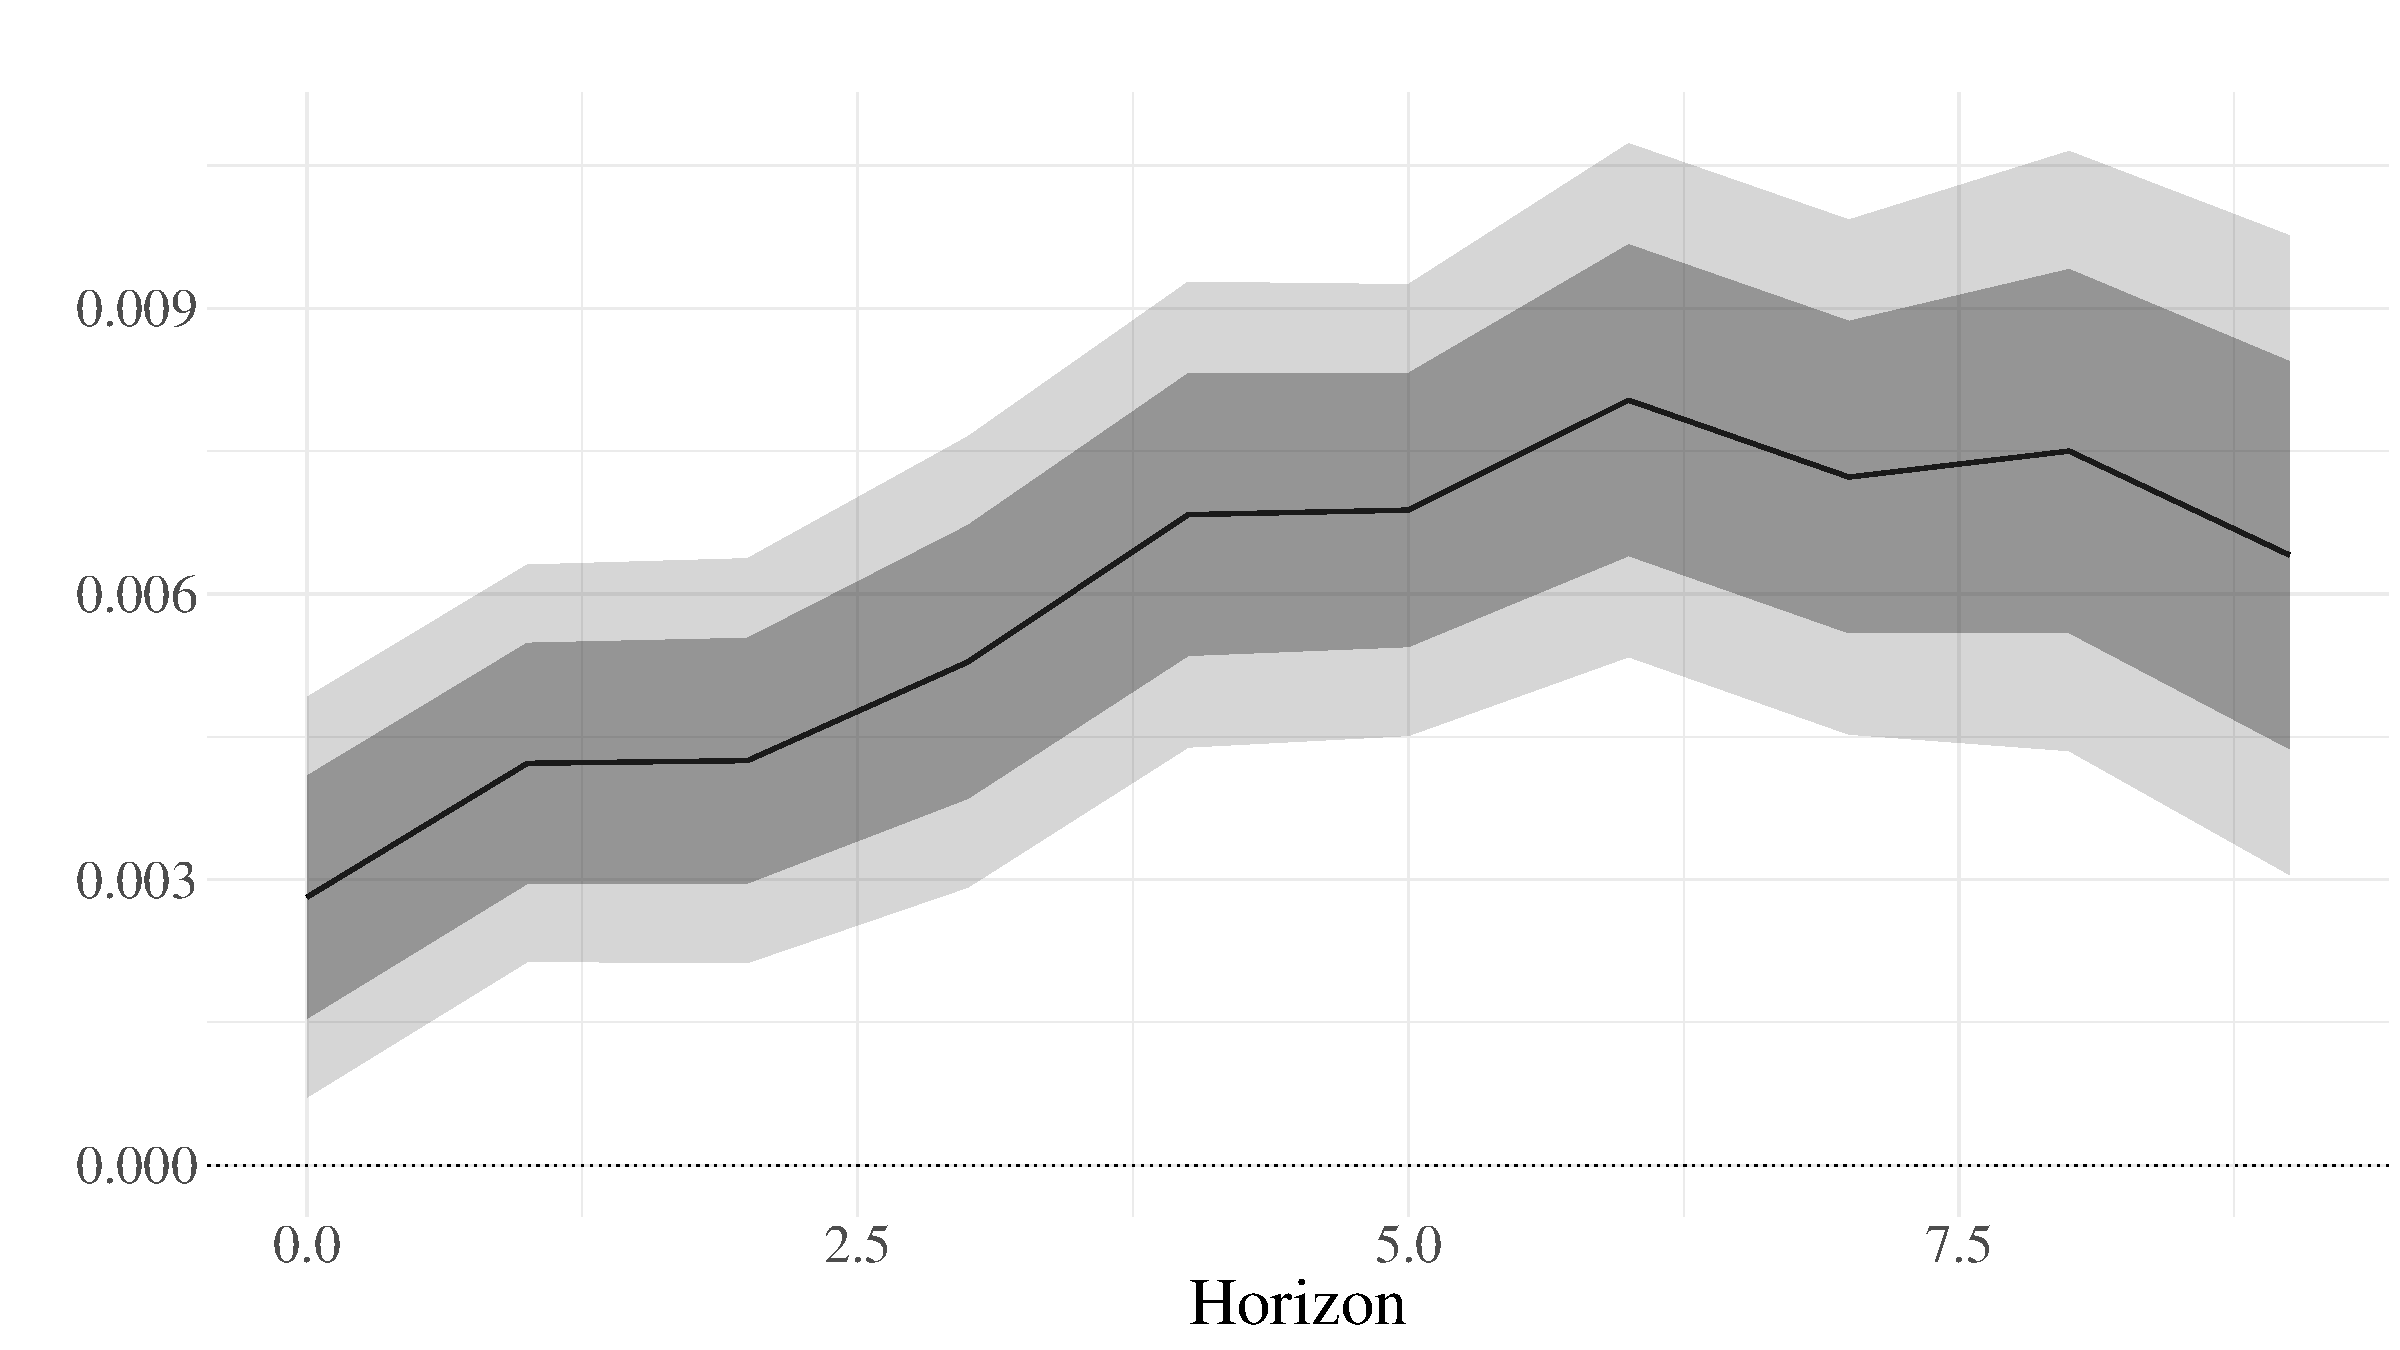
\includegraphics[width=.75\textwidth]{../figures/local_projections/patents_citations_resid.pdf}
\caption[Dynamic effect of value-weighted patents on $p_{it}$]{Dynamic effect of value-weighted patents on $p_{it}$ \footnotemark}
\label{fig:patents_citations_resid}
\end{figure}
\footnotetext{66\% confidence interval in dark grey, 90\% confidence interval in light. White standard errors.}

\subsubsection*{Robustness and Results Summary}

As a robustness check, I re-estimate my empirical specification limiting my sample to ``top suppliers'', i.e. the top-ten industry-input combinations in each year by expenditure share. My results are qualitatively unchanged. I also extend my sample, using historical data from the BEA stretching back to 1947, in Appendix \ref{ap:historical}. Again, my results are qualitatively unchanged. 

In sum, my parameter estimates confirm past work establishing the gross complementarity of intermediate inputs in US sectoral production, and document the following novel results\dots
\begin{enumerate}
    \item The ability of US industries to substitute inputs varies meaningfully across sectors (i.e. elasticities are heterogeneous across sectors in all years).
    \item The ability of US industries to substitute inputs varies meaningfully across time (i.e. elasticities are heterogenous across years in all sectors).
    \item The production functions of US industries evolve over time in ways that alter the relative ``importance'' of inputs (i.e. share parameters shift year-over-year).
\end{enumerate}

I will now turn to the implications of these results for the macroeconomy. 

% --------------------
\section{Quantitative Results}
\label{sec:discussion}
% --------------------

In this section I discuss the economic interpretation of my empirical results, and confirm their real-world relevance with a series of quantitative exercises.

My empirical results correspond to Scenarios 2, 2a, and 2b of the stylized example in Section \ref{subsec:stylized_example}. Sectoral heterogeneity in elasticities implies the macro effect of sectoral shocks will vary depending on the elasticities of the direct and indirect customers of the shocked sectors. Temporal heterogeneity in elasticities implies the macro effect of sectoral shocks will vary depending on the elasticities in the year of the shock. Temporal heterogeneity in share parameters implies the macro effect of sectoral shocks will vary depending on the importance of the shocked sectors as input suppliers in the year of the shock. 

To quantify these implied effects, I estimate the static general equilibrium defined in Section \ref{sec:theory}, calibrated to the US economy. I normalize prices and wages with respect to a base year; by default the base year is 2023. I define exogenous parameters as described in Table \ref{tab:calibration}.

\begin{table}[h]
    \centering
    \begin{threeparttable}
    \caption{Calibration of exogenous parameters}
    \begin{tabular}{|c|l|}
    \hline
    \textbf{Parameter} & \textbf{Calibration} \\ \hline
    $\alpha = \{\alpha_i\}$ & Value-added share at base year \\ \hline
    $\Omega = \{\omega_{ij}\}$ & Intermediate input expenditure share at base year \\ \hline
    $\mathcal{B} = \{\beta_i\}$ & Use market clearing condition, $\mathcal{B} = \mathcal{Y}_{gross} (I - \text{diag}(1-\alpha)\Omega)$\tnote{1} \\ \hline
    $\mathcal{L} = \{L_i\}$ & Use firm first-order condition, $\mathcal{L} = \alpha \mathcal{Y}_{gross} = \alpha(I - \text{diag}(1-\alpha)\Omega)^{-1} \mathcal{B}$ \\ \hline
    ${\sigma}$ & Set to .6 \tnote{2} \\ \hline
    $\nu$ & Set to .7 \tnote{3} \\ \hline
    \end{tabular}
    \begin{tablenotes}
    \footnotesize
    \item[1] Normalized to sum to 1.
    \item[2] See \citet{oberfieldMicroDataMacro2021} and \citet{carvalhoSupplyChainDisruptions2021}
    \item[3] See \citet{oberfieldMicroDataMacro2021}, Appendix Table I.3
    \end{tablenotes}
    \label{tab:calibration}
    \end{threeparttable}
\end{table}

\subsection{Macro effects with heterogenous elasticities} 

My first set of exercises quantify the macroeconomic implications of my elasticity results. I examine how my sector-varying elasticity estimates alter the predicted macro effect of severe shocks in individual sectors, and how my time-varying elasticity estimates alter the predicted macro effect of realistic shocks in all sectors.

I generate severe shocks to individual sectors as TFP shocks that cut sectoral output in half. I solve for the equilibrium corresponding to each shock, and store the resulting GDP. I perform this exercise with two elasticity calibrations: sector specific elasticities $\hat{\theta}^1_i$, and the corresponding average $\bar{\hat{\theta}}^1_i$ imposed across sectors.\footnote{Negative elasticity estimates are set to 0.001 in all exercises.}

In Table \ref{tab:extreme_shock_tab}, I list the 3 largest GDP reductions with sector-specific elasticities, and compare them with the corresponding results using the common elasticity.\footnote{In all tables, GDP effects are listed as the log-difference between no-shock GDP and shock GDP.} The difference between the two is due to how industries who directly and indirectly rely on the shocked sector for inputs deviate from the mean elasticity. For example, ``Primary metals'' is a relatively universal input, so a severe shock to the sector generates similar (large) GDP effects with heterogenous versus common sectoral elasticities. In contrast, ``Chemical products'' has direct and indirect customers with low elasticities relative to the average, so a severe shock to the sector generates a larger GDP effect when accounting for sectoral heterogeneity in elasticities: GDP falls by an additional $\approx 1.5$\%, an increase in magnitude of roughly $10\%$.

\begin{table}
    \centering
    \caption{GDP effect of severe sectoral shocks, 2023}
    \begin{tabular}{lccc}
\toprule
Industry Description & Sector-Specific & Uniform & Difference \\
\midrule
\midrule
\multicolumn{2}{l}{\textbf{Larger GDP loss}} \\
\midrule
Chemical products & -0.261 & -0.230 & -0.031 \\
Paper products & -0.059 & -0.046 & -0.013 \\
Oil and gas extraction & -0.066 & -0.062 & -0.003 \\
\midrule
\multicolumn{2}{l}{\textbf{Smaller GDP loss}} \\
\midrule
Insurance carriers and related... & -0.160 & -0.257 & 0.097 \\
Federal Reserve banks, credit ... & -0.161 & -0.177 & 0.016 \\
Primary metals & -0.094 & -0.101 & 0.007 \\
\bottomrule
\end{tabular}
    \label{tab:extreme_shock_tab}
\end{table}

To generate realistic shocks in all sectors, I use the Industry TFP measure reported in the BLS KLEMS data. I estimate the variance of annual and quadrennial sectoral TFP shocks from 1997-2023, and draw 1000 annual and 1000 quadrennial shocks from the corresponding multivariate normal distributions with mean 0.\footnote{I set off-diagonal elements of the covariance matrix to 0, though in practice this makes little difference as sectoral TFP shocks are mostly uncorrelated.} I assume labor is sector-specific and cannot move across industries, exogenously fixing $L_i$ at its calibrated value as reported in Table \ref{tab:calibration}. This is in line with existing empirical literature documenting little to no short-run labor reallocation across sectors in response to comparable shocks \citep{acemogluImportCompetitionGreat2016}.  I solve for the equilibrium corresponding to each shock, and store the resulting GDP.

I perform this exercise using a ``high'' elasticity calibration, where each sector's elasticity is set to the 75th percentile of its distribution across years, and a ``low'' elasticity calibration, where each sector's elasticity is set to the 25th percentile of its distribution across years. I also use a Cobb-Douglas calibration, as a benchmark. I compare the results, using annual and quadrennial shocks, in Table \ref{tab:shock_results} and Figure \ref{fig:shock_results_yearhet}. 

\begin{table}[!h]
    \centering 
    \caption{Logged GDP distributions}
    \label{tab:shock_results}
    
\begin{tabular}{lcccccc}
\toprule
& \multicolumn{3}{c}{Annual shocks} & \multicolumn{3}{c}{Quadrennial shocks} \\

\toprule
 & Mean & SD & Skewness & Mean & SD & Skewness \\
\midrule
Cobb-Douglas & -0.001 & 0.016 & 0.089 & -0.001 & 0.027 & 0.042 \\
High elasticity & -0.002 & 0.016 & 0.049 & -0.004 & 0.028 & 0.004 \\
Low elasticity & -0.003 & 0.016 & -0.001 & -0.010 & 0.028 & -0.037 \\
\bottomrule
\end{tabular}

\end{table}

\begin{figure}[!h]
    \centering 
    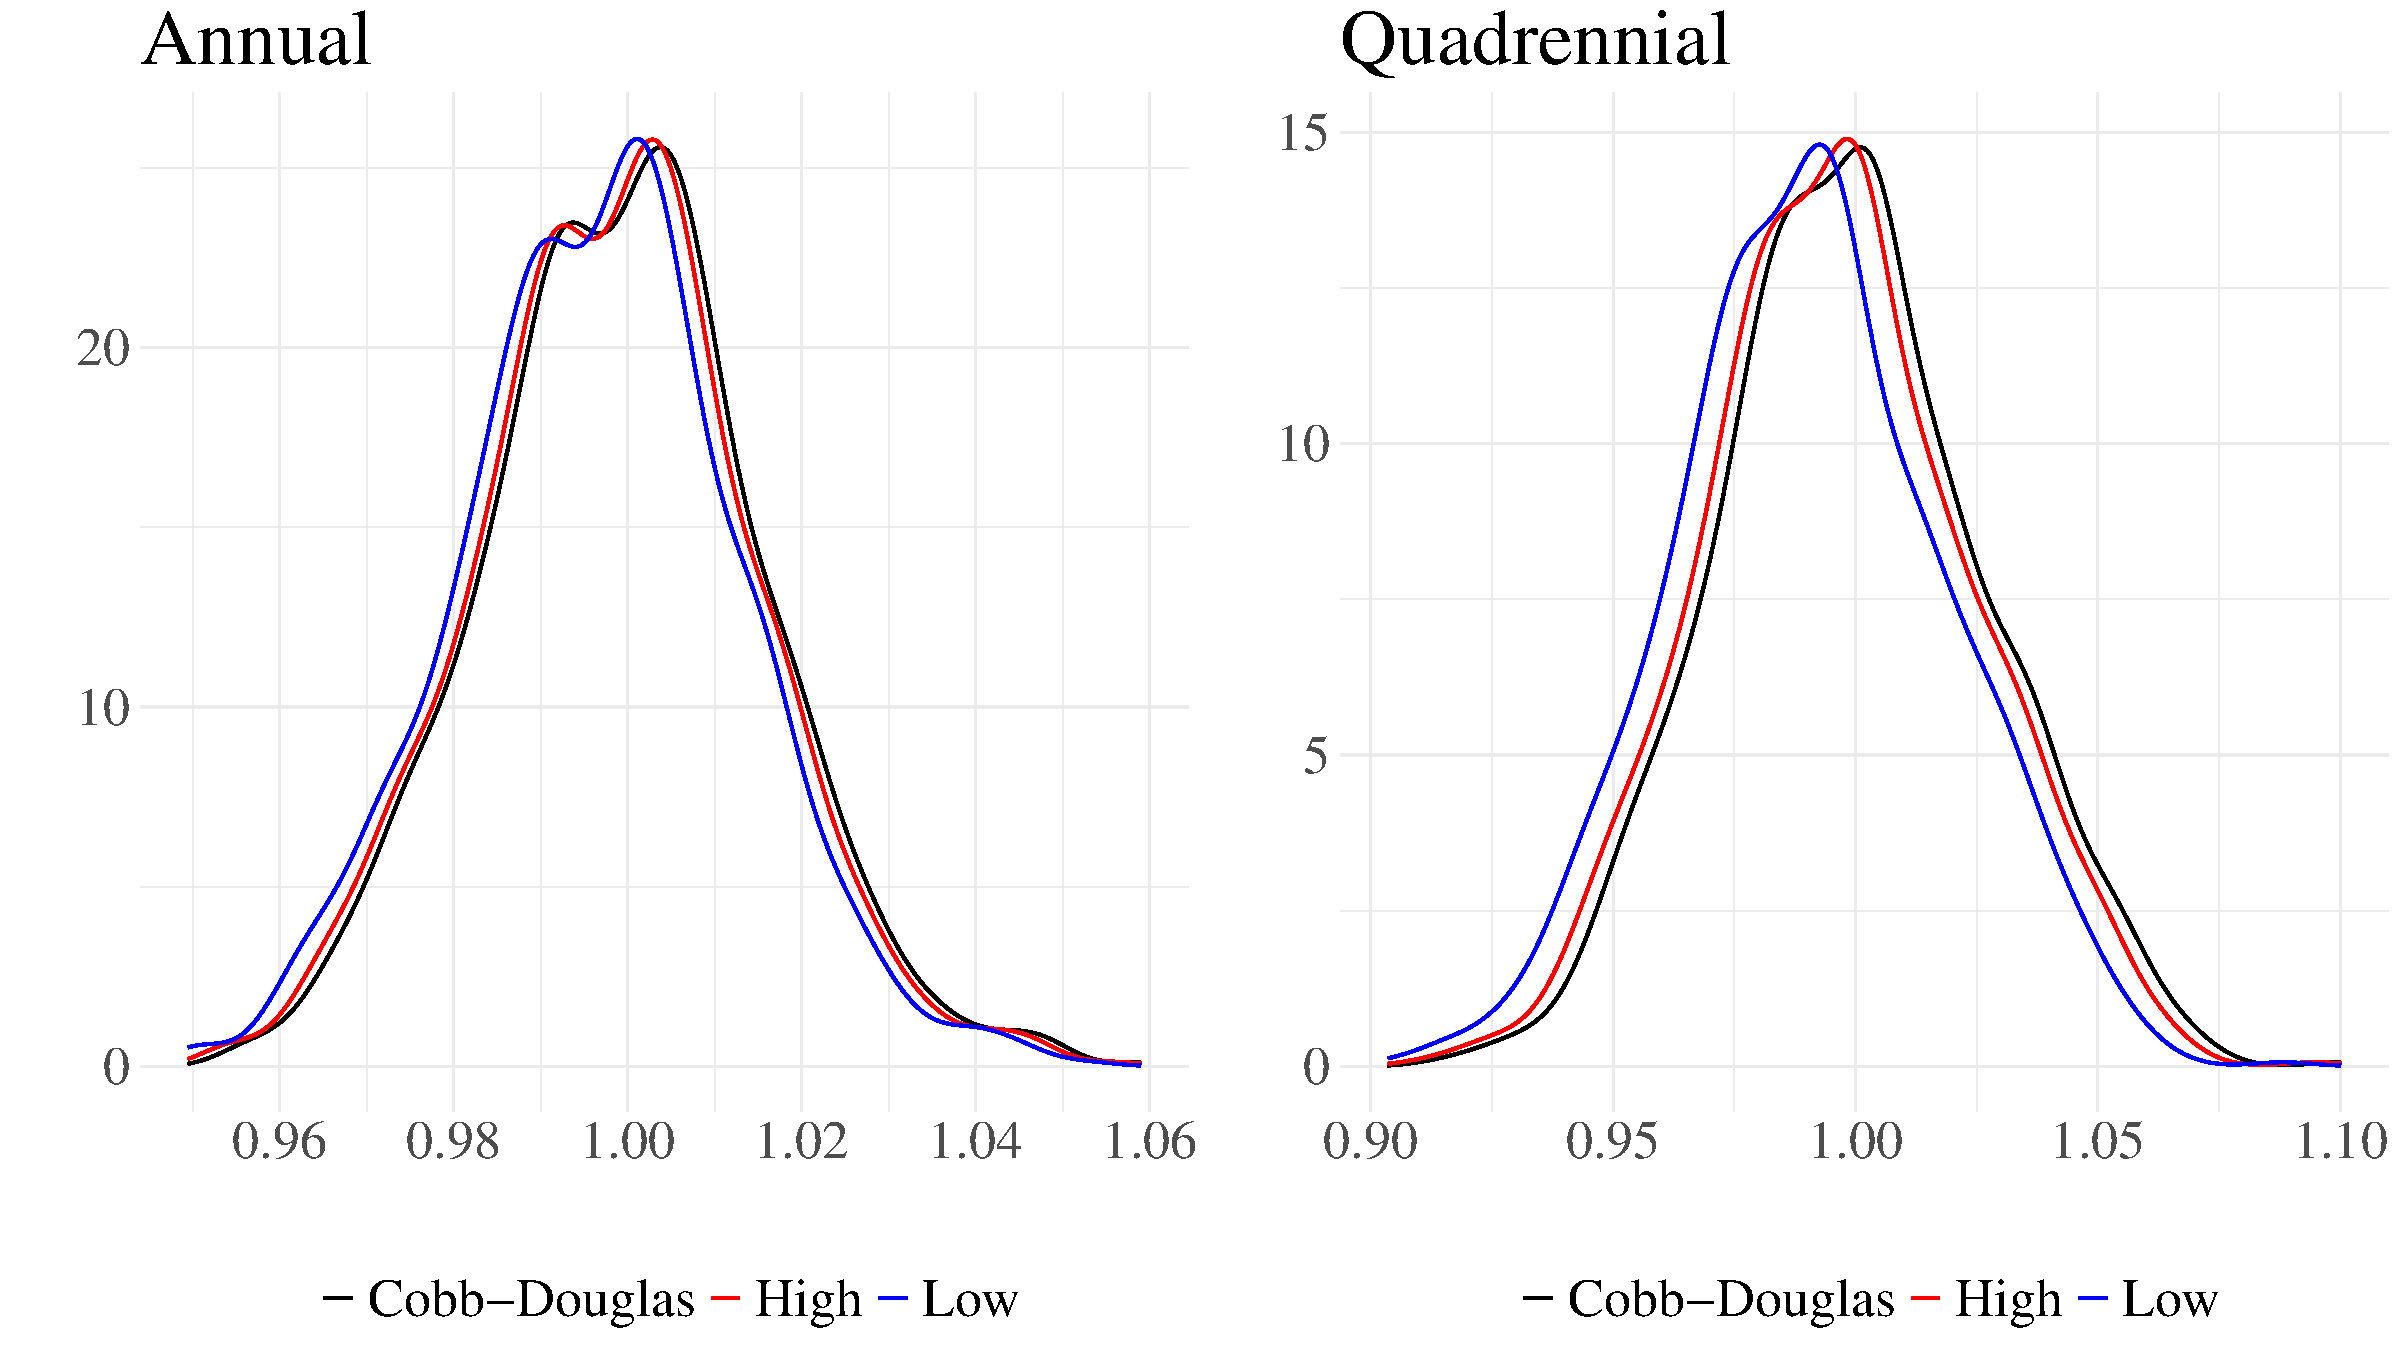
\includegraphics[width=\textwidth]{../figures/theory/gdp_het_year.pdf}
    \caption{GDP distributions with time-varying elasticities}
    \label{fig:shock_results_yearhet}
\end{figure}

As expected, complementarity across intermediate inputs amplifies the effect of negative micro shocks: both my empirical elasticity calibrations generate GDP distributions to the left of the Cobb-Douglas benchmark, with lower means and more negative skews. This pattern is exacerbated when moving from annual to quadrennial shocks: the larger TFP shocks generate greater non-linear propagation. 

However, the more meaningful difference quantitatively is between the ``high'' elasticity calibration and the ``low'' elasticity calibration. When simulating annual and quadrennial shocks, the difference in means and skews between the ``low'' and ``high'' GDP distributions exceeds the corresponding differences between the ``high'' and Cobb-Douglas GDP distributions. In other words, the macro implications of time-varying elasticities are quantitatively similar to the macro implications of gross complementarity across intermediate inputs. 

\subsection{Macro effects with time-varying share parameters} 

My second set of exercises quantify the macroeconomic implications of my share parameter results. As a validity check, I first examine how my estimates of share parameter shifts correspond with observed changes in sectoral output. I then examine how they alter the predicted macro effect of severe shocks in individual sectors.

For each year I observe share parameter shifts, I calibrate my model to be normalized with respect to the base period ($t-1$), once again assuming labor is sector-specific and therefore exogenously fixed. I simulate the effect of the estimated log-changes in share parameters in that year on equilibrium sectoral output. The relevant counterfactual is that the share parameters of each sectoral production function changed as implied by my estimates, but all other exogenous parameters stayed the same. I regress observed changes in sectoral output on the simulated changes: the resulting $R^2$ is $.09$. As a benchmark, I regress observed changes in sectoral output on sectoral TFP as well; the resulting $R^2$ is $.004$, suggesting that the GE effect of share parameter shifts is a far greater determinant of a sector's output than its own TFP. Results are summarized in Appendix Table \ref{tab:sector_output_prediction}

I also take the cumulative sum of the log changes in share parameters from 1997-2023. I set the base year to $1997$, and multiply my calibrated $\Omega_{1997}$ by these cumulative sums: the result is the share parameter matrix $\tilde{\Omega}_{2023}$.\footnote{I exponentiate the cumulative sum before multiplying, and additionally renormalize the share parameters to sum to 1.} The relevant counterfactual is that between 1997 and 2023 the share parameters of sectoral production functions changed as implied by my estimates, but all other exogenous parameters stayed the same. I calculate the equilibrium sectoral outputs corresponding to $\tilde{\Omega}_{2023}$. Due to the longer time horizon associated with this counterfactual, I report results with no labor reallocation across sectors ($L_i$ is exogenously fixed at its calibrated value, reported in Table \ref{tab:calibration}) and with full labor reallocation across sectors ($L_i$ is endogenously determined by equilibrium conditions; wages are equated across sectors). 

\begin{table}[!h]
    \centering 
    \caption{Sectoral output changes due to share parameter changes, 1997-2023}
    \label{tab:share_parameter_results}
    \begin{tabular}{lr}
\toprule
Industry Description & Output Growth, 1997-2023 \\
\midrule
Data processing, internet publishing, and other in... & 1.018 \\
Warehousing and storage & 0.995 \\
Computer systems design and related services & 0.645 \\
\bottomrule
\end{tabular}

\end{table}

The three largest increases in sectoral output under both sets of assumptions are reported in Table \ref{tab:share_parameter_results}. They largely line up with conventional wisdom. Information technology's increasingly central role in a broad range of sectors is reflected in large increases in the equilibrium sectoral output of ``Computer and electronic products'' and ``Data processing, internet publishing, and other information services'' driven by share parameter shifts across US industries between 1997 and 2023. As expected, the effects are greater when labor is allowed to reallocate across sectors freely.

Satisfied with this validity check, I examine how my estimated share parameter shifts between 1997 and 2023 alter the predicted macro effect of severe shocks to individual sectors. I again generate severe shocks to individual sectors as TFP shocks that cut sectoral output in half. I solve for the equilibrium corresponding to each shock, and store the corresponding GDP. I compare the results using the 1997 calibration of $\Omega_{1997}$ to the results using $\tilde{\Omega}_{2023}$. I allow labor to reallocate in response to the share parameter shifts, but not in response to the sectoral shocks.\footnote{In practice, this is implemented as two shocks. The first shock is the share parameter shifts, with full labor reallocation; I store the resulting GDP $Y_1^{noshock}$ and labor allocation. The second shock is the TFP shock, with no labor reallocation; I store the resulting GDP $Y_1^{shock}$ and report differences as $\log(Y_1^{shock}) - \log(Y_1^{noshock})$.} 

\begin{table}[!h]
    \centering 
    \caption{Change in GDP effect of severe sectoral shocks, 1997 to 2023}
    \label{tab:severe_shock_tab_1997_2023}
    \begin{tabular}{lccc}
\toprule
Industry Description & ${\Omega}_{2023}$ & $\tilde{\Omega}_{1997}$ & Difference \\
\midrule
\midrule
\multicolumn{2}{l}{\textbf{Larger GDP loss}} \\
\midrule
Other real estate & -0.133 & -0.106 & -0.027 \\
Data processing, internet publ... & -0.039 & -0.014 & -0.025 \\
Management of companies and en... & -0.069 & -0.049 & -0.020 \\
\midrule
\multicolumn{2}{l}{\textbf{Smaller GDP loss}} \\
\midrule
Chemical products & -0.261 & -0.334 & 0.074 \\
Oil and gas extraction & -0.066 & -0.121 & 0.056 \\
Federal Reserve banks, credit ... & -0.161 & -0.202 & 0.041 \\
\bottomrule
\end{tabular}
\end{table}

In Table \ref{tab:severe_shock_tab_1997_2023}, I list the three sectors with the largest increases and decreases in GDP effect using $\tilde{\Omega}_{2023}$ versus $\Omega_{1997}$. My results demonstrate how share parameter shifts between 1997 and 2023 altered the predicted macro effect of severe shocks in individual sectors. In particular, changes in the product functions of sectors have made ``Computer and electronic products'' a more central direct and indirect supplier of inputs, resulting in a larger macro effect of a severe shock to the sector. The same is true, to a lesser degree, for the ``Chemical products'' and ``Data processing'' sectors. In contrast, those same changes have made ``Paper products'' a less central direct and indirect supplier of inputs, resulting in a smaller macro effect of a severe shock to the sector. 

Note that the same comparison using 1997 and 2023 as the baseline years will not perfectly correspond with the results in Table \ref{tab:severe_shock_tab_1997_2023}. The reason is that the data used to calibrate the model in both periods imply changes in exogenous parameters beyond $\Omega$. For example, as computers and electronic products have become cheaper, they have become a smaller share of household expenditure, implying a smaller $\beta_i$. Thus while the indirect macro effect (via sector-to-sector propagation) of a shock to the ``Computer and electronic products'' sector has magnified, the direct effect (via household direct expenditures) has fallen. I use the counterfactual $\tilde{\Omega}_{2023}$ for this reason, to isolate the effect of changes in the relative importance of inputs in sectoral production functions on micro-to-macro propagation. 

\begin{table}[!h]
    \centering 
    \caption{Change in GDP effect of severe sectoral shocks, 2023 to 2033}
    \label{tab:severe_shock_tab_2023_2033}
    \begin{tabular}{lccc}
\toprule
Industry Description & $\lvert \Delta \text{GDP}(\tilde{\Omega}_{2033}) \rvert - \lvert \Delta \text{GDP}(\Omega_{2023}) \rvert$ \\
\midrule
\midrule
\multicolumn{2}{l}{\textbf{Largest increases in GDP effect}} \\
\midrule
Management of companies and enterprises & 0.021 \\
Warehousing and storage & 0.017 \\
Data processing, internet publishing, and other in... & 0.013 \\
\midrule
\multicolumn{2}{l}{\textbf{Largest decreases in GDP effect}} \\
\midrule
Chemical products & -0.018 \\
Paper products & -0.014 \\
Insurance carriers and related activities & -0.012 \\
\bottomrule
\end{tabular}
\end{table}

Finally, I use my estimated share parameter shifts to predict the macro effects of severe sectoral shocks in the future. I use share parameter shifts over the last ten years to generate $\tilde{\Omega}_{2033}$. The relevant counterfactual is assuming share parameter shifts follow the same (linear) trend between 2023 and 2033 as they did between 2013 and 2023, while all other exogenous parameters remain fixed. I again allow labor to reallocate in response to the share parameter shifts, but not in response to the severe sectoral shocks. I list the three largest increases and decreases in the resulting macro effect in Table \ref{tab:severe_shock_tab_2023_2033}. Negative shocks to ``Warehousing and storage'', ``Management of companies and enterprises'', and ``Data processing, internet publishing, and other information services'', are predicted to have larger macro effects, due to their increasingly central role in the production of other goods. Conversely, the macro effects of negative shocks to ``Chemical products'', ``Paper products'', and ``Insurance  carriers and related activities'' are predicted to fall. 



\section*{Conclusion}

In this paper, I revisit the classic question of the micro-to-macro propagation of sectoral shocks. The answer to this question depends on the ability of sectors to substitute inputs in production and the relative importance of sectors as direct and indirect suppliers of inputs. I demonstrate that in standard models of production, these features depend on two sets of parameters: the elasticity of substitution across intermediate inputs, and the share parameters of sectoral production functions. I relax the restrictive assumptions of existing estimates of these parameters, permitting them to vary across industries and across time, by using a novel empirical strategy that relies on the unique within-industry/across-input variation provided by the BEA input-output accounts. My estimates document novel facts about US sectoral production: (1) the ability of US industries to substitute inputs varies meaningfully across sectors, (2) the ability of US industries to substitute inputs varies meaningfully across time, and (3) the production functions of US industries evolve over time in ways that alter the relative ``importance'' of inputs. I quantify the macroeconomic implications of these results using a calibrated general equilibrium model of the US economy. I show that all three results meaningfully alter the macro effect of sectoral shocks. 

My paper leaves several avenues for future research, of which I highlight two. First, while the focus of the paper is the macro effect of negative shocks to sectoral TFP, my results have more general implications. The elasticity of substitution and industry-input share parameters determine how sectors respond to changes in input price. Thus the sector-to-sector propagation of any economic phenomena that manifests in prices will be effected by heterogeneity in these parameters, including distortions \citep{bigioDistortionsProductionNetworks2020} and price rigidities \citep{rubboNetworksPhillipsCurves2023} \citep{laoOptimalMonetaryPolicy2022}. I leave these implications for future research.

Second, I treat time-variation in elasticities and share parameters as exogenous. However, given the large changes in these parameters across time, and the quantitatively meaningful implications of these changes, understanding \textit{why} these parameters change is an important unanswered question. In particular, the large year-to-year swings in elasticities, which imply very different micro-to-macro propagation, is a puzzle worth exploring in models endogenizing the parameter. I leave this to future research.

\pagebreak 

% %%%%%%%%%%%%%%%%%%%%%%%%%%%%%%%%%%%%%%%%%%%%%%%%%%%%%%%%%%
% %%%%%%%%%%%%%%%%%%%%%%%%%%%%%%%%%%%%%%%%%%%%%%%%%%%%%%%%%%
% APPENDIX
% %%%%%%%%%%%%%%%%%%%%%%%%%%%%%%%%%%%%%%%%%%%%%%%%%%%%%%%%%%
% %%%%%%%%%%%%%%%%%%%%%%%%%%%%%%%%%%%%%%%%%%%%%%%%%%%%%%%%%%
\appendix
\renewcommand{\thefigure}{A.\arabic{figure}}
\setcounter{figure}{0}
\renewcommand{\thetable}{A.\arabic{table}}
\setcounter{table}{0}

\section{Appendix}
% make subsections A.

\subsection{Relation to \citet{atalayHowImportantAre2017} and \citet{miranda-pintoFlexibilityFrictionsMultisector2022}}
\label{ap:atalay}
% label as ap:atalay

As described above, \citet{atalayHowImportantAre2017} and \citet{miranda-pintoFlexibilityFrictionsMultisector2022} also expenditure share shifts to estimate the elasticity of substitution across intermediate inputs. My approaches differ on two fronts: (1) I use updated data which covers more industries (66 versus 30) and more years (1997-2023 versus 1997-2013), and (2) I solely estimate ``inner-nest'' parameters, which allows me to use variation across industry-input-years for my estimates rather than rely on instruments that vary at the industry-year level. While (1) is straightforward, (2) is worth discussing in more detail.

\citet{atalayHowImportantAre2017} and \citet{miranda-pintoFlexibilityFrictionsMultisector2022} estimate both the inner-nest elasticity across intermediate inputs $\theta$ and the outer-nest elasticity between value-added production and intermediate inputs $\sigma$ using changes in relative price and expenditure shares. To do so, they derives a reduced form by combining the first-order conditions of the cost-minimization problem with respect to the intermediate input bundle $M_i$ and good $X_{ij}$\dots

\[
\begin{aligned}
\frac{Q_i M_i}{C_i Y_i} = (1-\alpha_i) Z_i^{\sigma_i - 1} \left(\frac{Q_i}{C_i}\right)^{1 - \sigma_i} \rightarrow \partial \log \left(\frac{Q_i M_i}{C_i Y_i}\right) = (\sigma_i - 1) \partial \log(Z_i) + (1 - \sigma_i) \partial \log \left(\frac{Q_i}{C_i}\right) \\
\frac{P_j X_{ij}}{Q_i M_i} = \omega_{ij} \left(\frac{P_j}{Q_i}\right)^{1 - \theta_i} \rightarrow \partial \log \left(\frac{P_j X_{ij}}{Q_i M_i}\right) = (1 - \theta_i) \partial \log \left(\frac{P_j}{Q_i}\right) \\
\partial \log \left(\frac{P_j X_{ij}}{C_i Y_i}\right) = (1 - \theta_i) \partial \log \left(\frac{P_j}{Q_i}\right) + (\sigma_i - 1) \partial \log(Z_i) + (1 - \sigma_i) \partial \log \left(\frac{Q_i}{C_i}\right)
\end{aligned}
\]

Note that share parameters are assumed to be constant ($\partial \log \alpha_i = \partial \log \omega_{ij} = 0$) and mark-ups are assumed to be constant ($\partial \log C_i = \partial \log P_i$). This reduced form regression can identiy inner-nest elasticities $\theta_i$ and outer-nest elasticities $\sigma_i$ with variation in expenditure shares and prices, if Hicks neutral technology $Z_i$ is controlled for. Unfortunately, we cannot control for this term using industry-year fixed effects, since the relative price of the intermediate input bundle $\frac{Q_i}{C_i}$, which provides identifying variation for $\sigma_i$, is constant within an industry-year. The intuition is that while the cost-share of specific intermediate inputs $X_{ij}$ offer 66 first-order conditions to estimate $\theta_i$, the cost-share of the overall intermediate input bundle $M_i$ offers only 1. 

To get around this issue, \citet{atalayHowImportantAre2017} constructs three instruments using year-over-year shifts in military spending, the revenue share of the general federal government defense sector (GFGD), and the row-sums of the Leontief inverse of the input-output ``customer'' matrix.\footnote{\citet{miranda-pintoFlexibilityFrictionsMultisector2022} use the same instruments. Formal definitions can be seen in both papers.} While these instruments satisfy the exclusion restriction, they also vary at the industry-year level, meaning they eliminate the industry-input-year variation that my estimates isolate (and that are unique to the BEA input-output accounts). 

As an exercise, I construct the Atalay instruments, and estimate my empirical specification (imposing constant elasticity $\theta$ across industries and years as in \citet{atalayHowImportantAre2017}) using these instruments. I compare the results to my main estimates, which use industry-year fixed effects. The results are summarized in Table \ref{tab:atalay_comparison} and Appendix Table \ref{tab:atalay_comparison_subset}. Note that in Appendix Table \ref{tab:atalay_comparison_subset}, my Atalay IV estimates more precisely match the empirical strategy of \citet{atalayHowImportantAre2017}: I use revenue shares instead of cost shares and I estimate the outer-nest elasticity as the (transformed) coefficient on the log-change of the ratio of intermediate input bundle price and output price. I also only use data from 1997-2013 and only include observations of from the top ten suppliers of each industry for both sets of estimates in Appendix Table \ref{tab:atalay_comparison_subset}.

While the point estimates are (comfortingly) similar, the standard errors are much larger in the Atalay specification. This is especially true when clustering at the industry-year level, a reasonable choice given the nature of the identifying variation when using the Atalay instruments. The lost precision makes it impossible to recover more granular estimates of $\theta$ using the Atalay instruments. Moreover, the Atalay approach requires directly observing $Q_i$ via the Fisher index of the intermediate input bundle. Since a Fisher index requires the CES aggregator to have constant parameters in adjacent periods, it is also impossible to recover share parameter shifts $\Delta \log \omega_{ijt}$ using the Atalay approach.

\subsection{Extending sample using historical data}
\label{ap:historical}

In addition to the modern series used in the main analysis, the BEA provides historical data on input-output accounts and GDP by industry, from 1947-1996. I use this data to construct a longer sample of sectoral expenditure shares and relative price changes, using the same approach as described in Section 2. However, \textbf{I separate this sample into three periods: 1947-1962, 1963-1996, and 1997-2023}. This separation is due to the non-harmonized nature of the data. I estimate my empirical specification on the extended sample, producing estimates of the elasticity of substitution across intermediate inputs $\hat{\theta}^1_{it}$ and share parameter shifts $\Delta \log \omega_{ijt}$ from 1948-1962, 1964-1996, and 1998-2023. 

Since the KPSS data extends back to 1926, I can perform the same Jorda regressions as in the main analysis using my extended sample share parameter shifts; the results are visible in Figure \ref{fig:patents_value_resid_hist} and Figure \ref{fig:patents_citations_resid_hist}, and are qualitatively similar to the main results, further validating my empirical strategy. My extended sample elasticites are summarized in Figures \ref{fig:theta_byCode_hist} and \ref{fig:theta_byYear_hist}. As in my main analysis, my elasticity estimates demonstrate (A) broad complementarity and (B) meaningful heterogeneity across industries and across years. 

The extended sample allows for some descriptive analysis of correspondence between elasticity estimates and economic history, best visualized in Figure \ref{fig:theta_byYear_hist}. The low elasticity estimates in the early-to-mid 1970s correspond well with the 1973-1974 energy crisis, and more broadly the stagflation of the decade: both suggest a fragile economy sensitive to shifts in input prices and by extension domestic sectoral shocks. The high elasticities in the early-to-mid 1990s have the same quality: the period was marked by an economic boom, in part driven by an increase in trade, both of which rationalize a robust economy with abundant cheap inputs preventing major propagation of domestic sectoral shocks. Finally, the sharp drops in elasticity from 1999 to 2000/2001, and from 2006 to 2007, seem to correspond to the 2000-2001 recession and the 2007-2009 financial crisis, respectively.

In contrast, the negative mean elasticities from 1985-1989, the significantly negative mean elasticity in 2011, and the absence of any visible Covid shock in 2021-2022, all are harder to rationalize. I leave these as open questions for future research.

\subsection{Solving Vertical Supply Chain example}
\label{ap:stylized_example}

Suppose sectoral production follows a vertical supply chain. The output of each sector is CES aggregate of the output of the sector preceding it in the chain, and a sector specific good $X_{i1}$. These sector specific goods are exogenously fixed at some quantity greater than the output of the preceding sector. 

To understand propagation in this setting, I solve for the log change in $Y_i$ resulting from a log change in sectoral output $Y_{i-1}$. I do this by combining the production technology conditions with market clearing conditions\dots

\[
\begin{aligned}
Y_i = Z_i \left(\omega_{i1}^{1/\theta_i} X_{i1}^{\frac{\theta_i - 1}{\theta_i}} + \omega_{i2}^{1/\theta_i} Y_{i-1}^{\frac{\theta_i - 1}{\theta_i}}\right)^{\frac{\theta_i}{\theta_i - 1}} \\
\partial Y_i/\partial Y_{i-1} = Z_i^{1-1/\theta_i} Y_i^{1/\theta_i}\ \omega_{i2}^{1/\theta_i} Y_{i-1}^{-1/\theta_i} \\
\frac{\partial \log Y_i}{\partial \log Y_{i-1}} = \frac{\partial Y_i/Y_i}{\partial Y_{i-1}/Y_{i-1}} = Z_i^{1-1/\theta_i} Y_i^{1/\theta_i-1} \omega_{i2}^{1/\theta_i} Y_{i-1}^{1-1/\theta_i} \\
\frac{\partial \log Y_i}{\partial \log Y_{i-1}} = \omega_{i2}^{1/\theta_i} \left( \frac{Y_{i-1}^{\frac{\theta_i-1}{\theta_i}}}{\omega_{i1}^{1/\theta_i} X_{i1}^{\frac{\theta_i - 1}{\theta_i}} + \omega_{i2}^{1/\theta_i} Y_{i-1}^{\frac{\theta_i - 1}{\theta_i}}} \right)
\end{aligned}
\]

When $\theta_i=1$, this collapses to the standard Cobb-Douglas case, where propagation is log-linear with coefficient $\omega_{i2}$. When $\theta_i > 1$, observe that\dots

\[
\begin{aligned}
\omega_{i1}^{1/\theta_i} X_{i1}^{\frac{\theta_i - 1}{\theta_i}} + \omega_{i2}^{1/\theta_i} Y_{i-1}^{\frac{\theta_i - 1}{\theta_i}} > Y_{i-1}^{\frac{\theta_i - 1}{\theta_i}}(\omega_{i1}^{1/\theta_i} + \omega_{i2}^{1/\theta_i}) \\
\frac{\partial \log Y_i}{\partial \log Y_{i-1}} < \frac{\omega_{i2}^{1/\theta_i}}{\omega_{i1}^{1/\theta_i} + \omega_{i2}^{1/\theta_i} }
\end{aligned}
\] 

Thus, when $\theta_i = 2$ and $\omega_{i1} = \omega_{i2} = 1/2$, as in Scenario 2a\dots

\[
\frac{\partial \log Y_{i}}{\partial \log Y_{i-1}} < \frac{\sqrt{1/2}}{\sqrt{1/2} + \sqrt{1/2}} = 1/2
\]

Delivering the result that a sectoral shock to cutting output of sector $N/2$ by $10$\% has a macro-effect of $-X$\% in even periods, where $X < 10 \times (1/2)^{N/2}$.


\pagebreak

\section*{Appendix Tables}

\begin{table}[!h]
    \centering 
    \caption{Comparison with \citet{atalayHowImportantAre2017}}
    \label{tab:atalay_comparison_subset}
    
\begin{tabular}{l c c c c}
\hline
 & \multicolumn{2}{c}{Robust SE} & \multicolumn{2}{c}{Clustered SE} \\
\cline{2-3} \cline{4-5}
 & Uniform & Atalay IV & Uniform & Atalay IV \\
\hline
Elasticity (inner-nest) & $0.18$   & $0.16$   & $0.18$   & $0.16$   \\
                        & $(0.05)$ & $(0.24)$ & $(0.05)$ & $(0.24)$ \\
Elasticity (outer-nest) &          & $1.30$   &          & $1.30$   \\
                        &          & $(0.48)$ &          & $(1.02)$ \\
\hline
\end{tabular}

\end{table}

\begin{table}[!h]
    \centering
    \caption{Predictive power of simulated changes in sectoral output}
    
\begin{tabular}{l c c}
\hline
 & \multicolumn{2}{c}{Observed change in sectoral output} \\
\cline{2-3}
 & Simulated change & Sectoral TFP \\
\hline
Coefficient & $0.97^{***}$ & $0.13^{**}$ \\
            & $(0.07)$     & $(0.05)$    \\
\hline
R$^2$       & $0.09$       & $0.00$      \\
Adj. R$^2$  & $0.09$       & $0.00$      \\
Num. obs.   & $1716$       & $1716$      \\
\hline
\multicolumn{3}{l}{\scriptsize{$^{***}p<0.001$; $^{**}p<0.01$; $^{*}p<0.05$}}
\end{tabular}

    \label{tab:sector_output_prediction}
\end{table}

\pagebreak 

% --------------------
\section*{Appendix Figures}
% --------------------

\begin{figure}[!h]
\centering
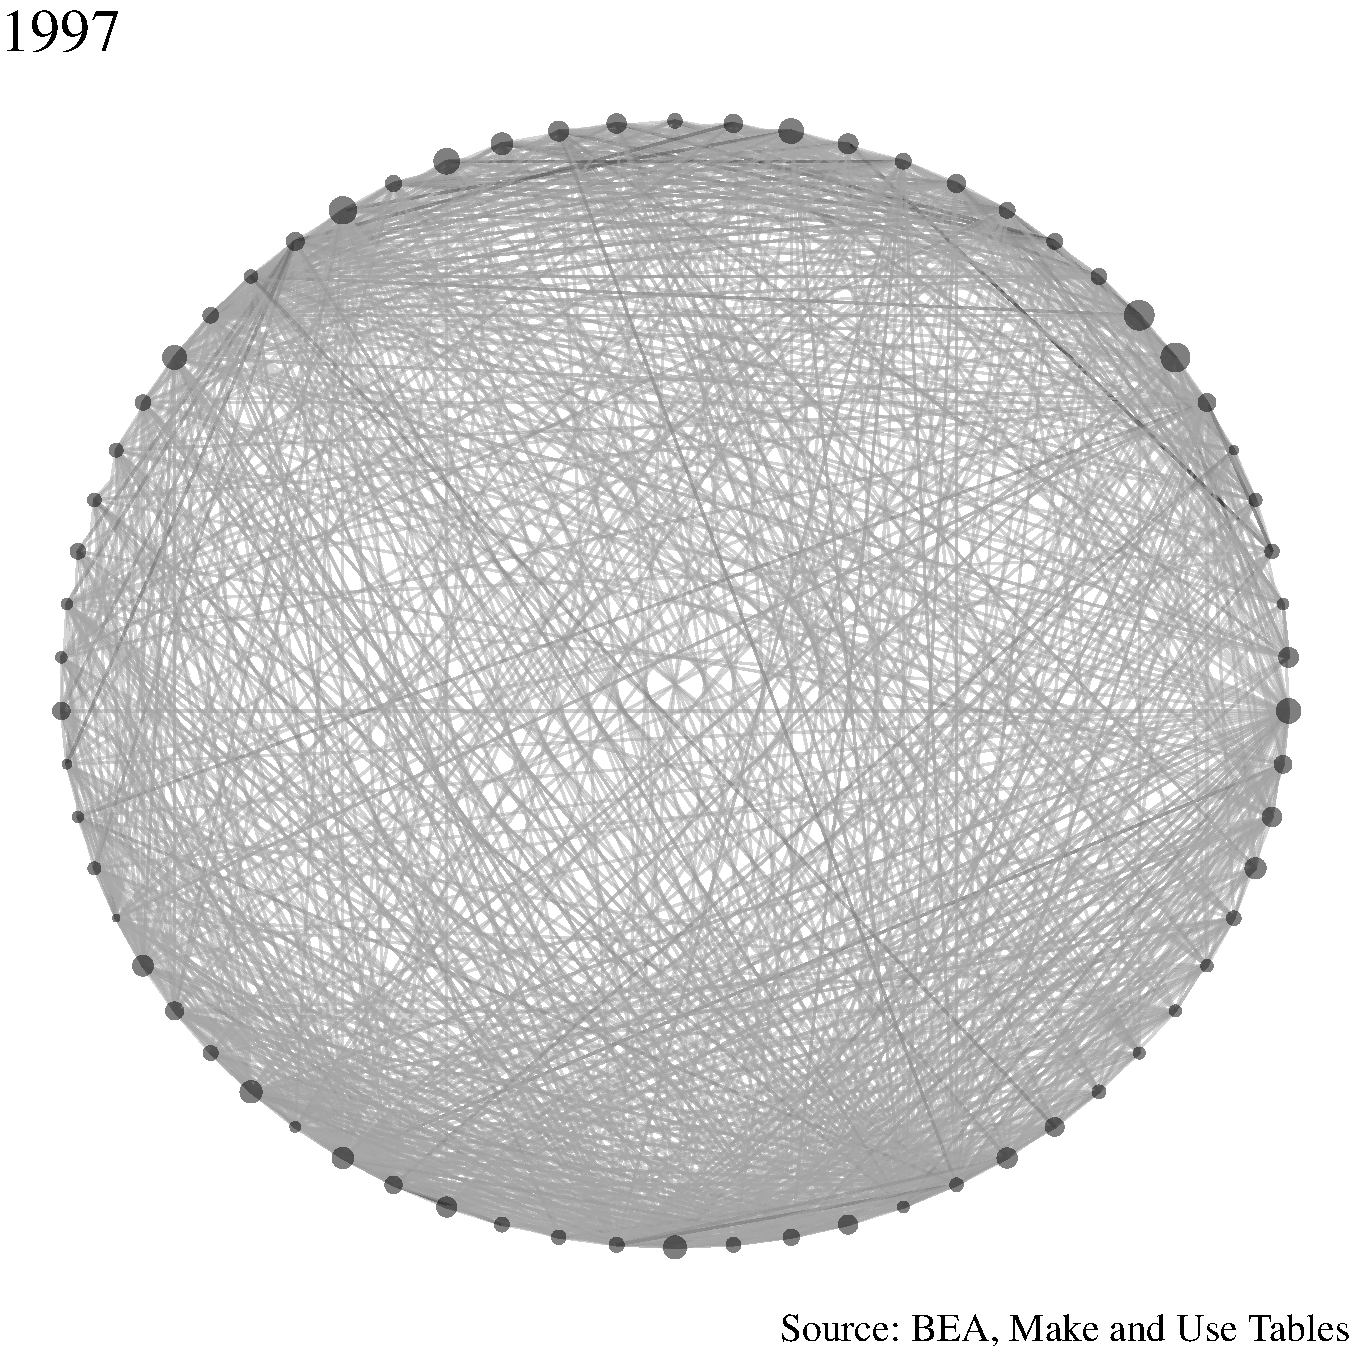
\includegraphics[width=.65\textwidth]{../figures/digraphs/A_summary_1997.pdf}
\caption{Production network in 1997}
\label{fig:PN1997}
\end{figure}

\begin{figure}
\centering
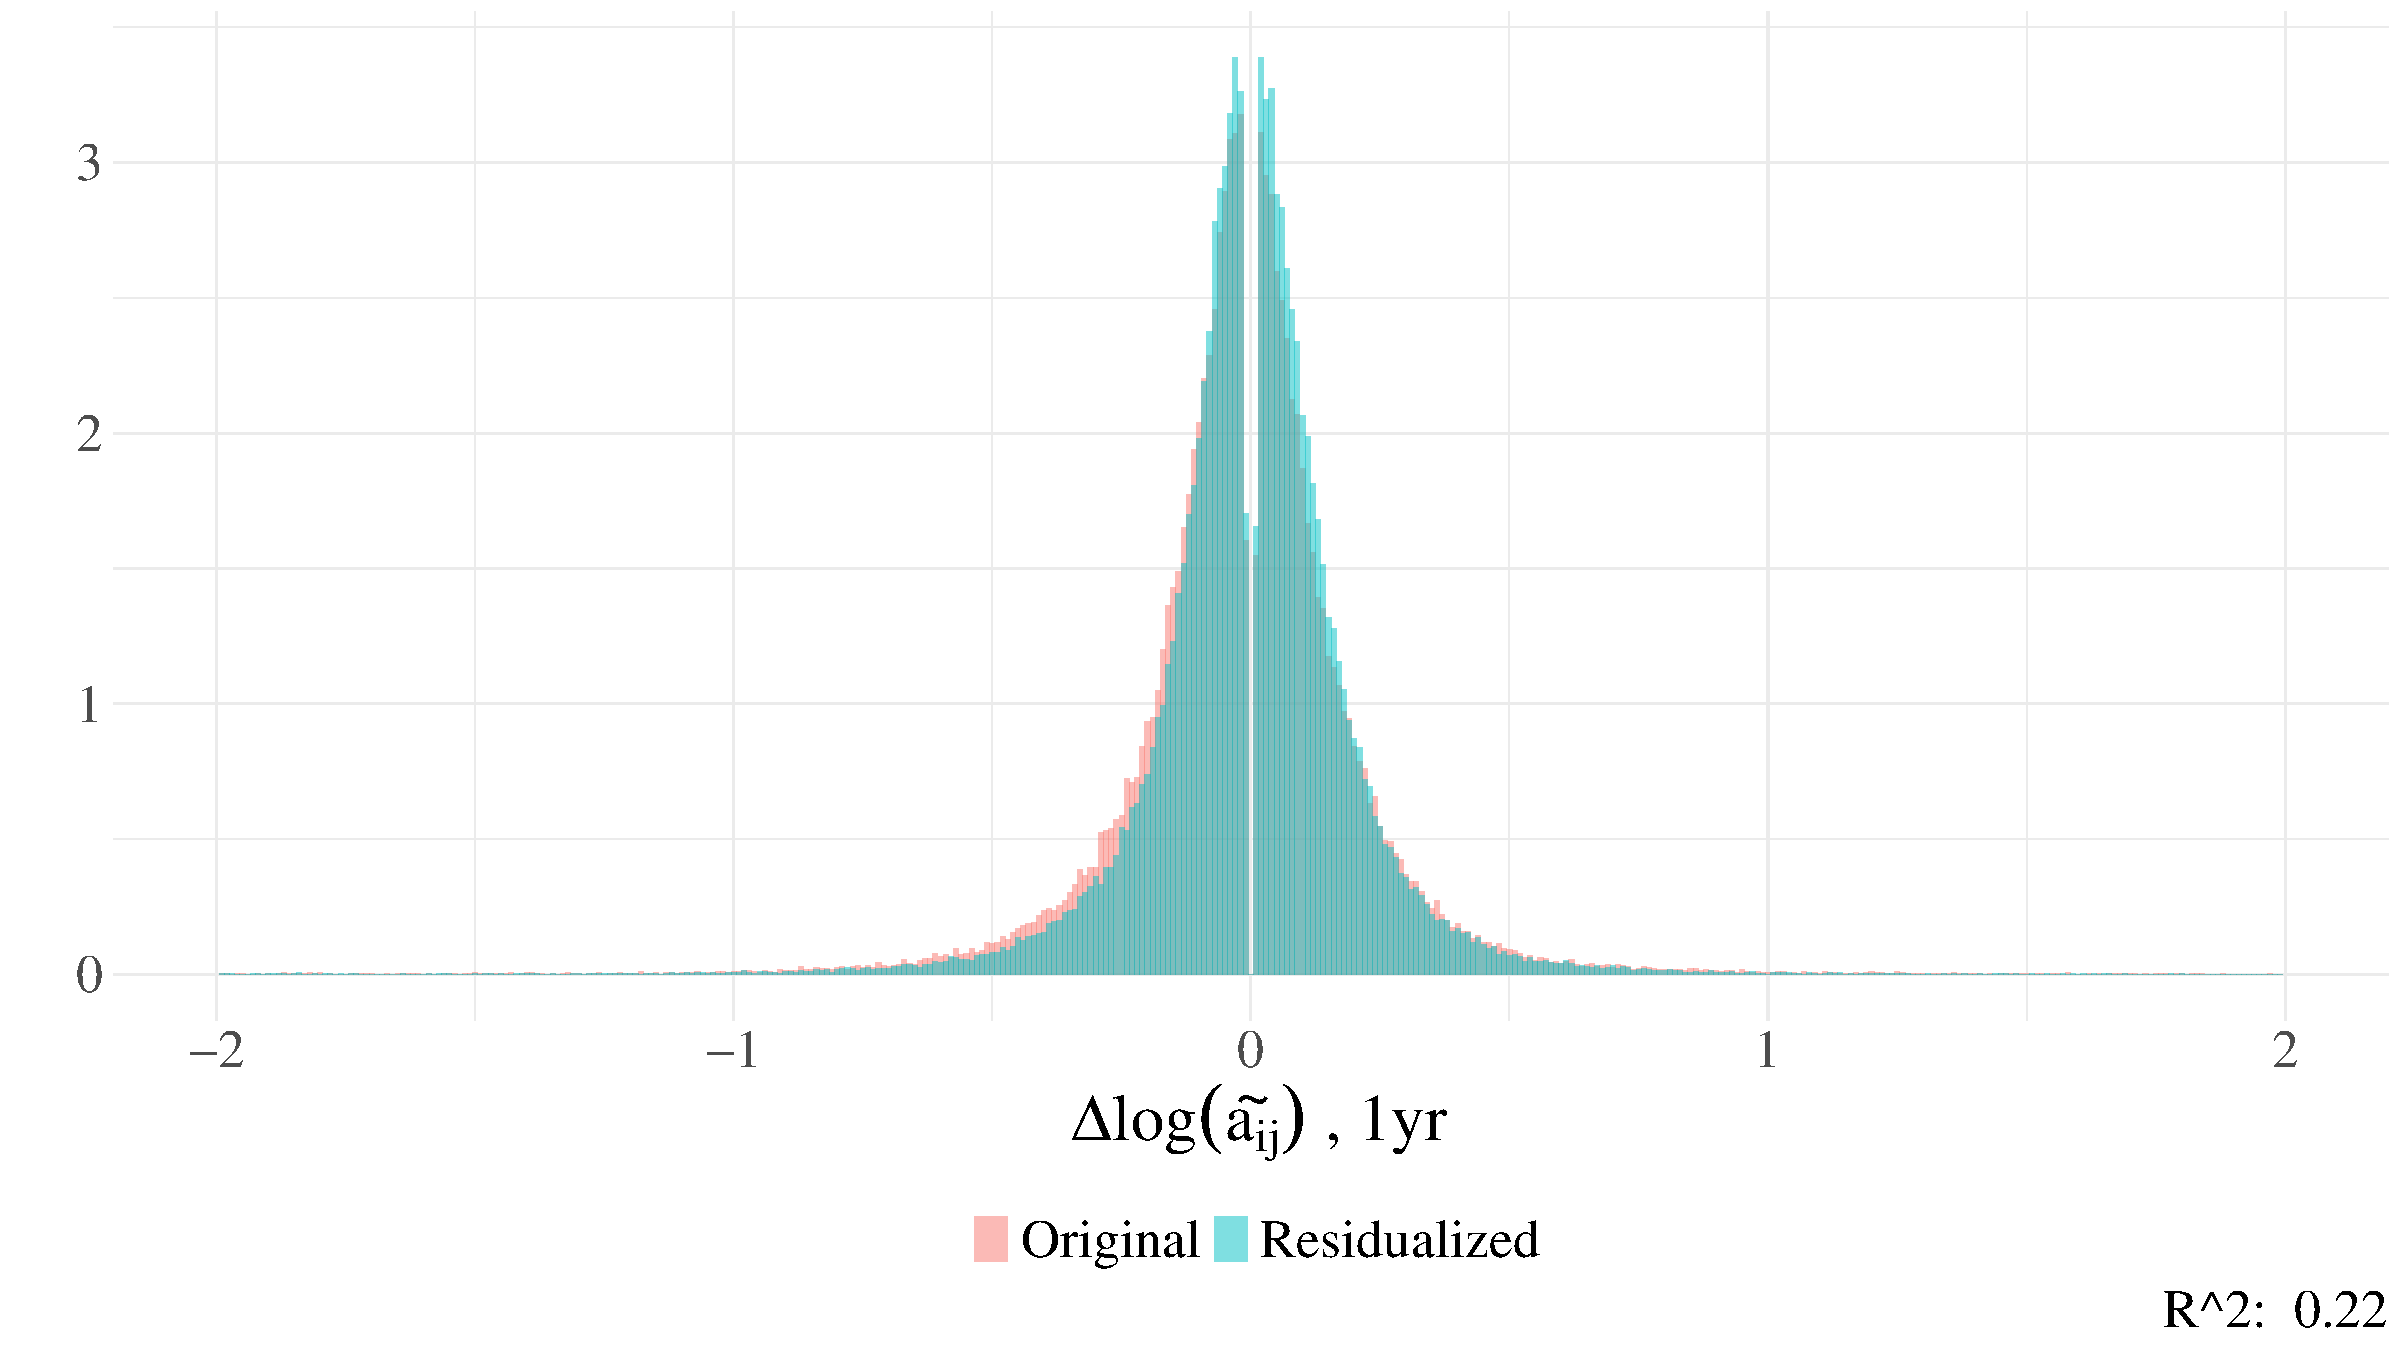
\includegraphics[width=.75\textwidth]{../figures/histograms/resid_hist.pdf}
\caption{Residuals of empirical specification}
\label{fig:reg_resid}
\end{figure}

\begin{figure}
\centering 
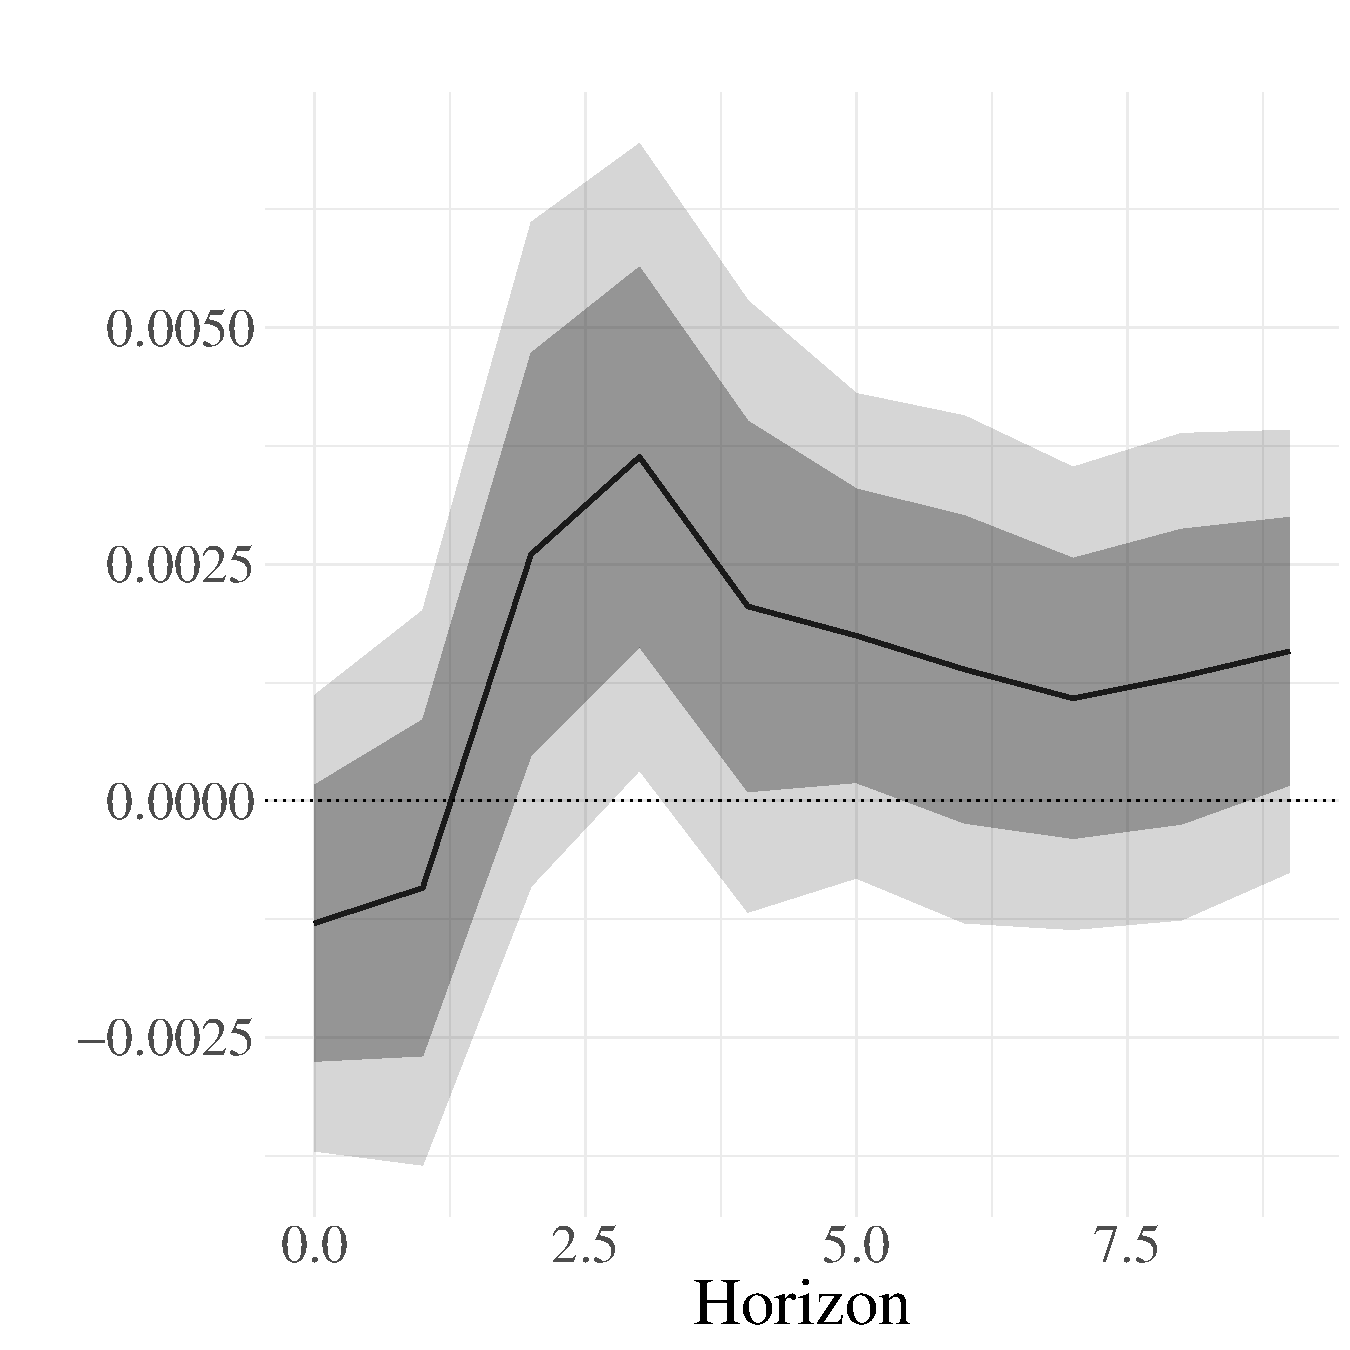
\includegraphics[width=.75\textwidth]{../figures/local_projections/patents_value_resid.pdf}
\caption{Dynamic effect of value-weighted patents on $p_{it}$}
\label{fig:patents_value_resid}
\end{figure}

\begin{figure}
\centering 
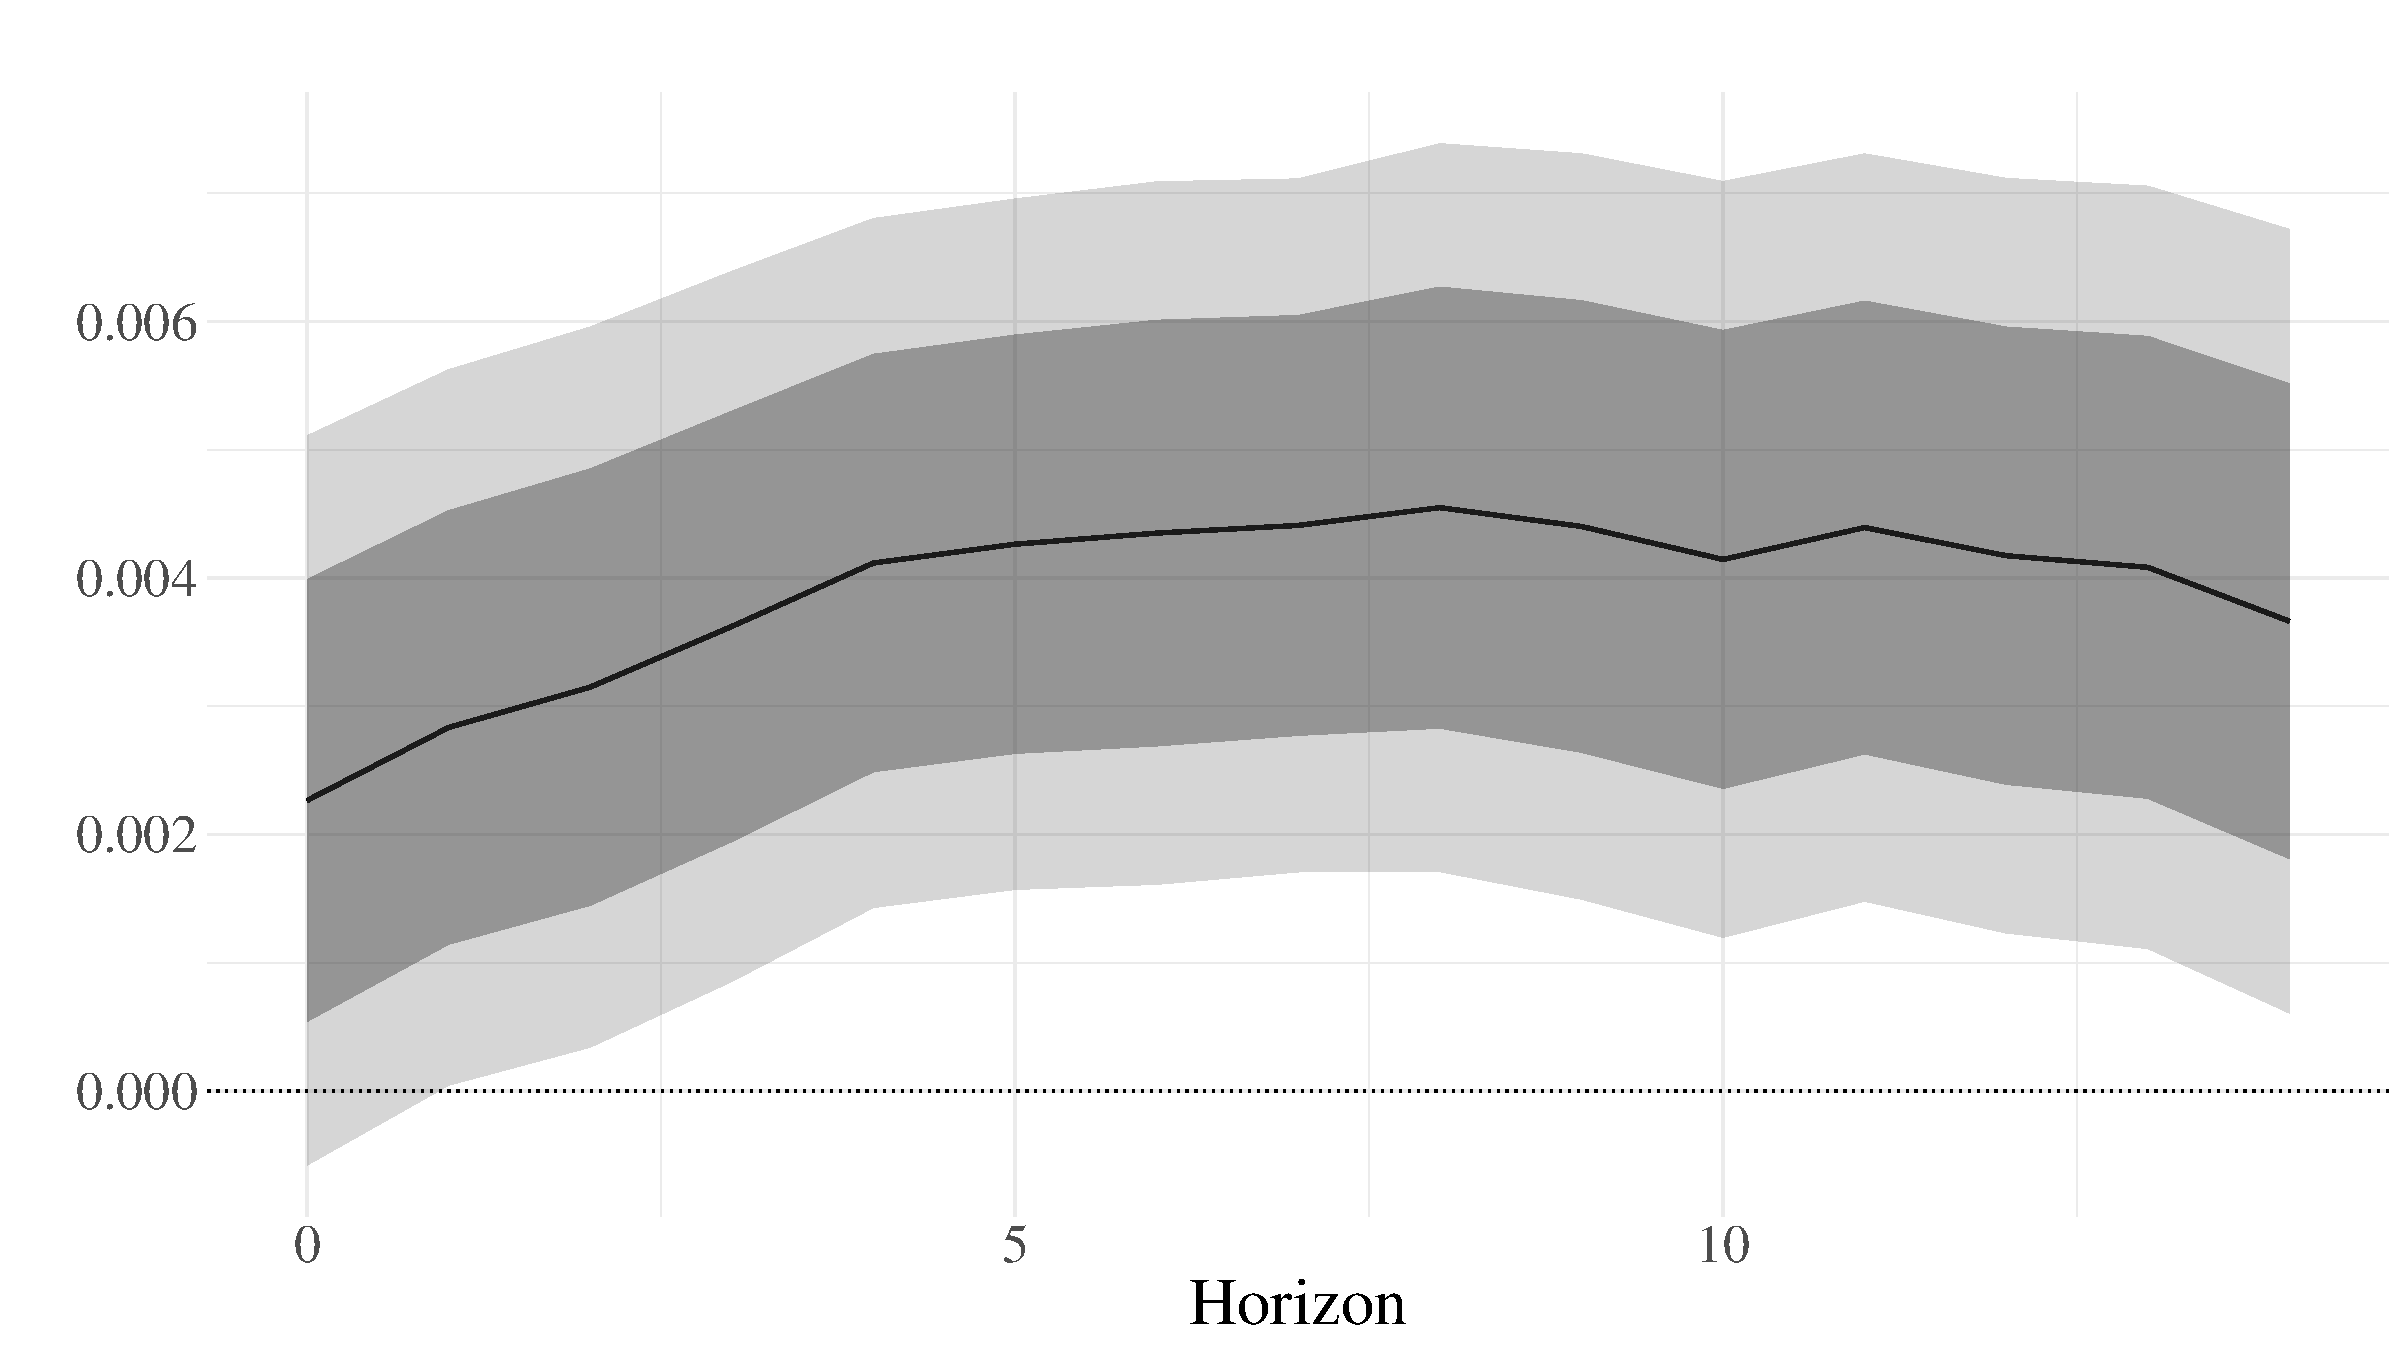
\includegraphics[width=.75\textwidth]{../figures/local_projections/patents_citations_resid_hist.pdf}
\caption{Dynamic effect of citation-weighted patents on $p_{it}$, extended sample}
\label{fig:patents_citations_resid_hist}
\end{figure}

\begin{figure}[!h]
\centering 
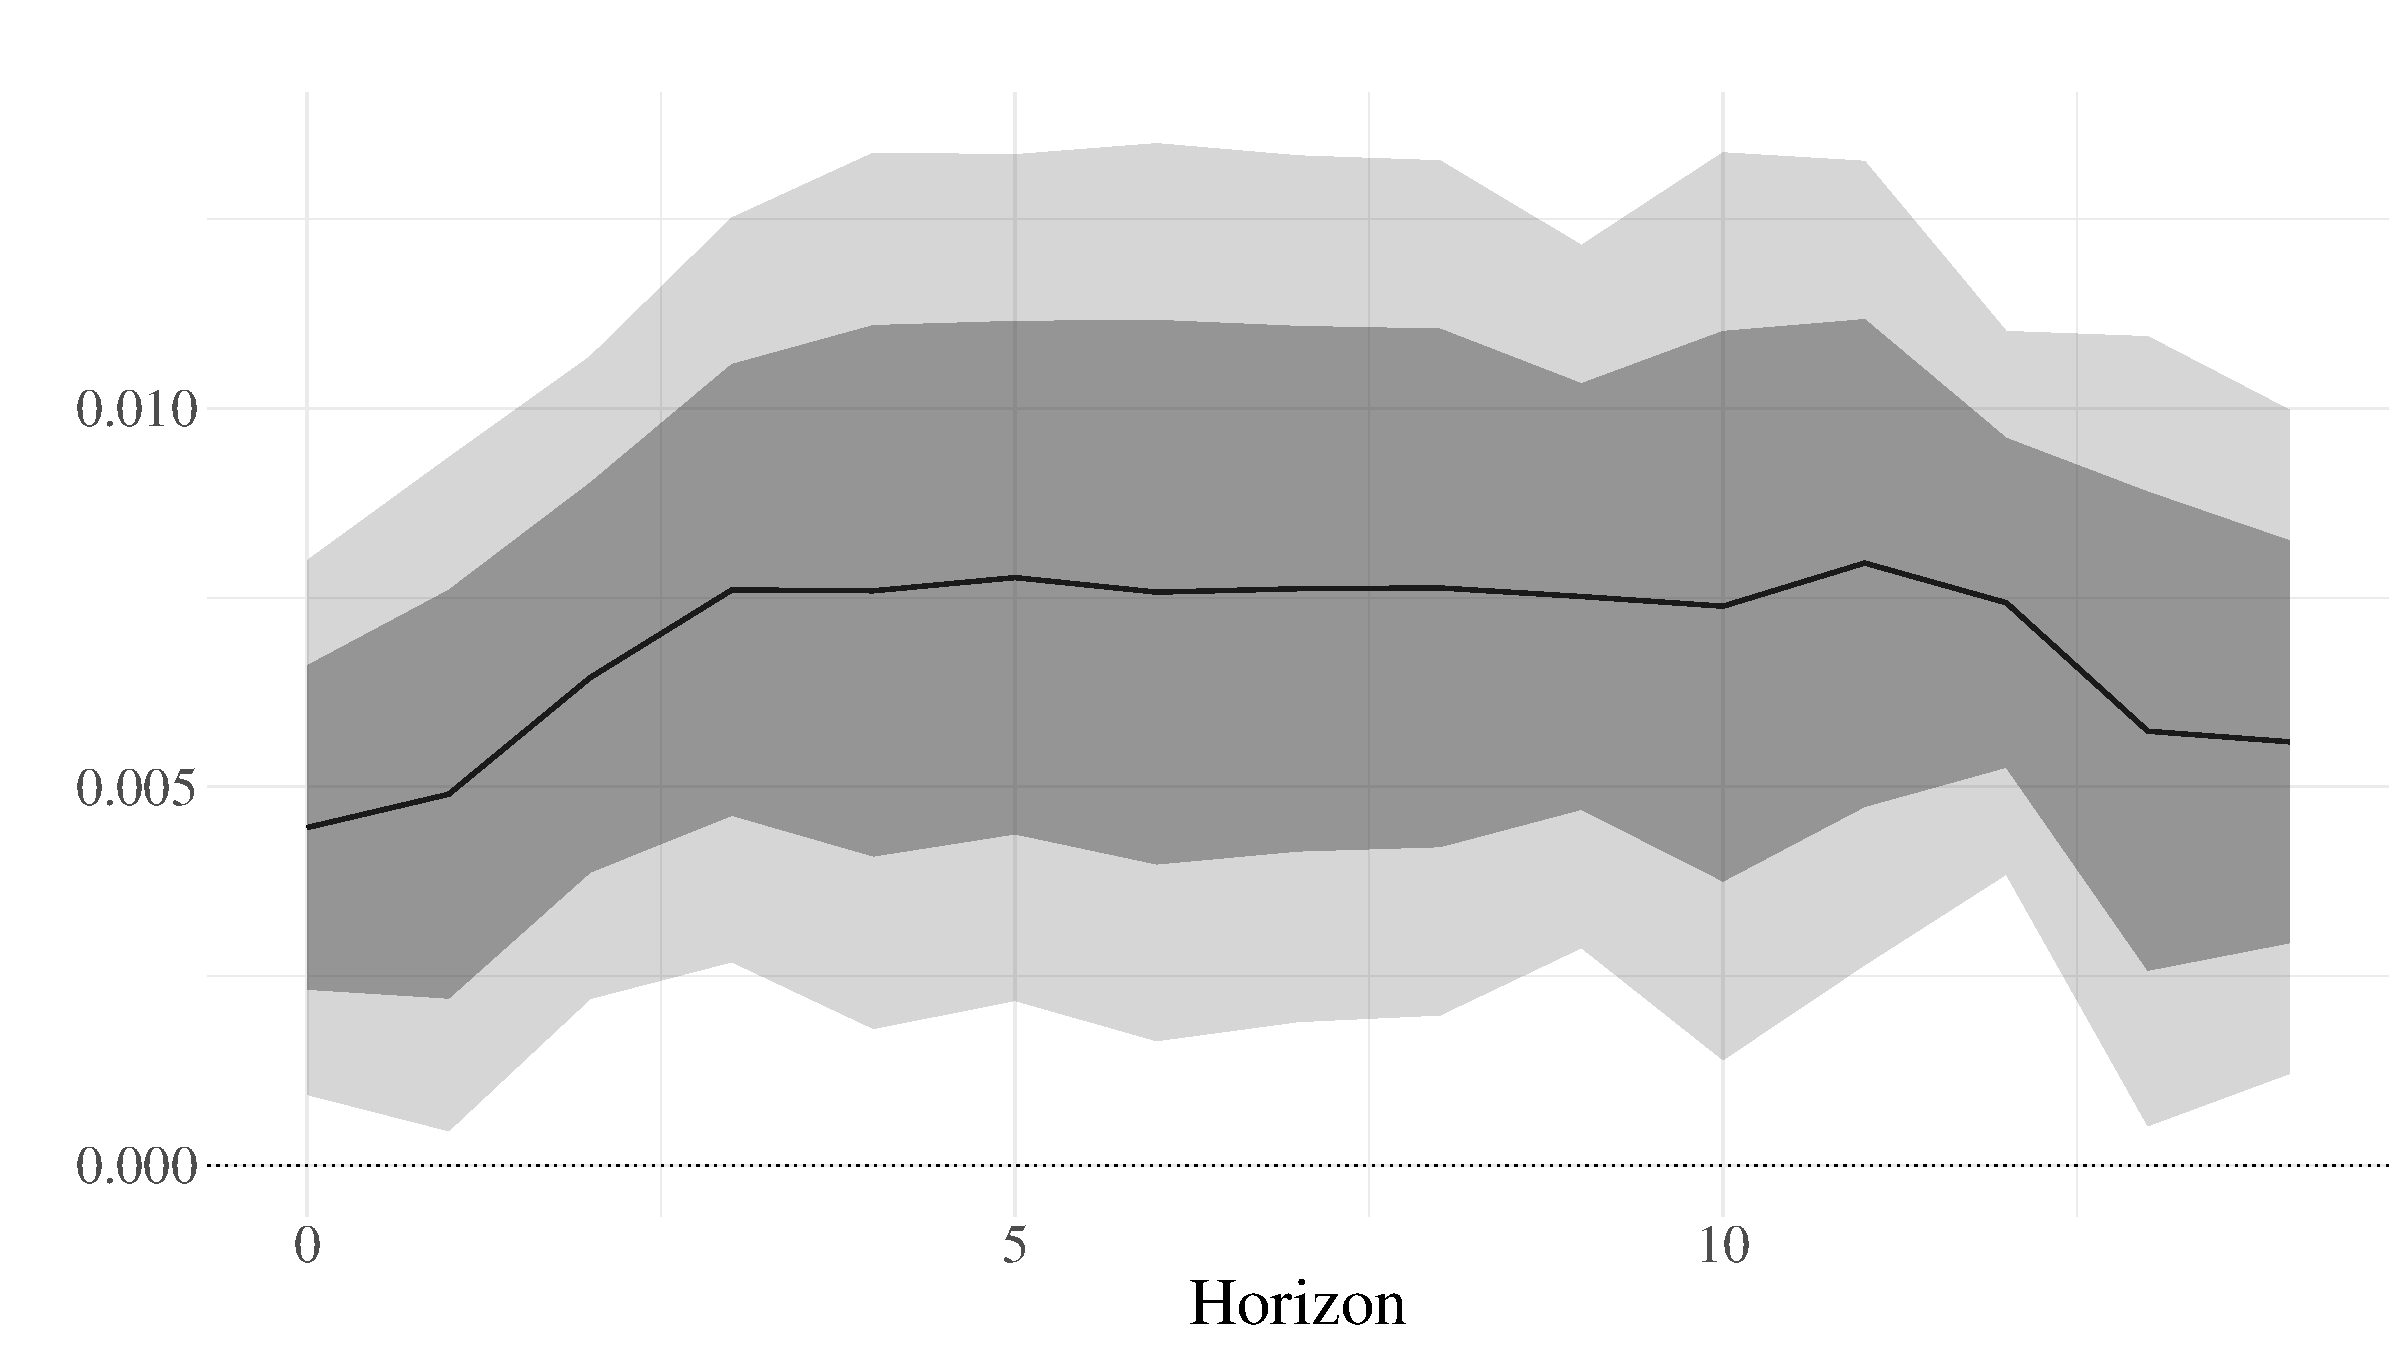
\includegraphics[width=.75\textwidth]{../figures/local_projections/patents_value_resid_hist.pdf}
\caption{Dynamic effect of value-weighted patents on $p_{it}$, extended sample}
\label{fig:patents_value_resid_hist}
\end{figure}

\begin{figure}[!h]
\centering
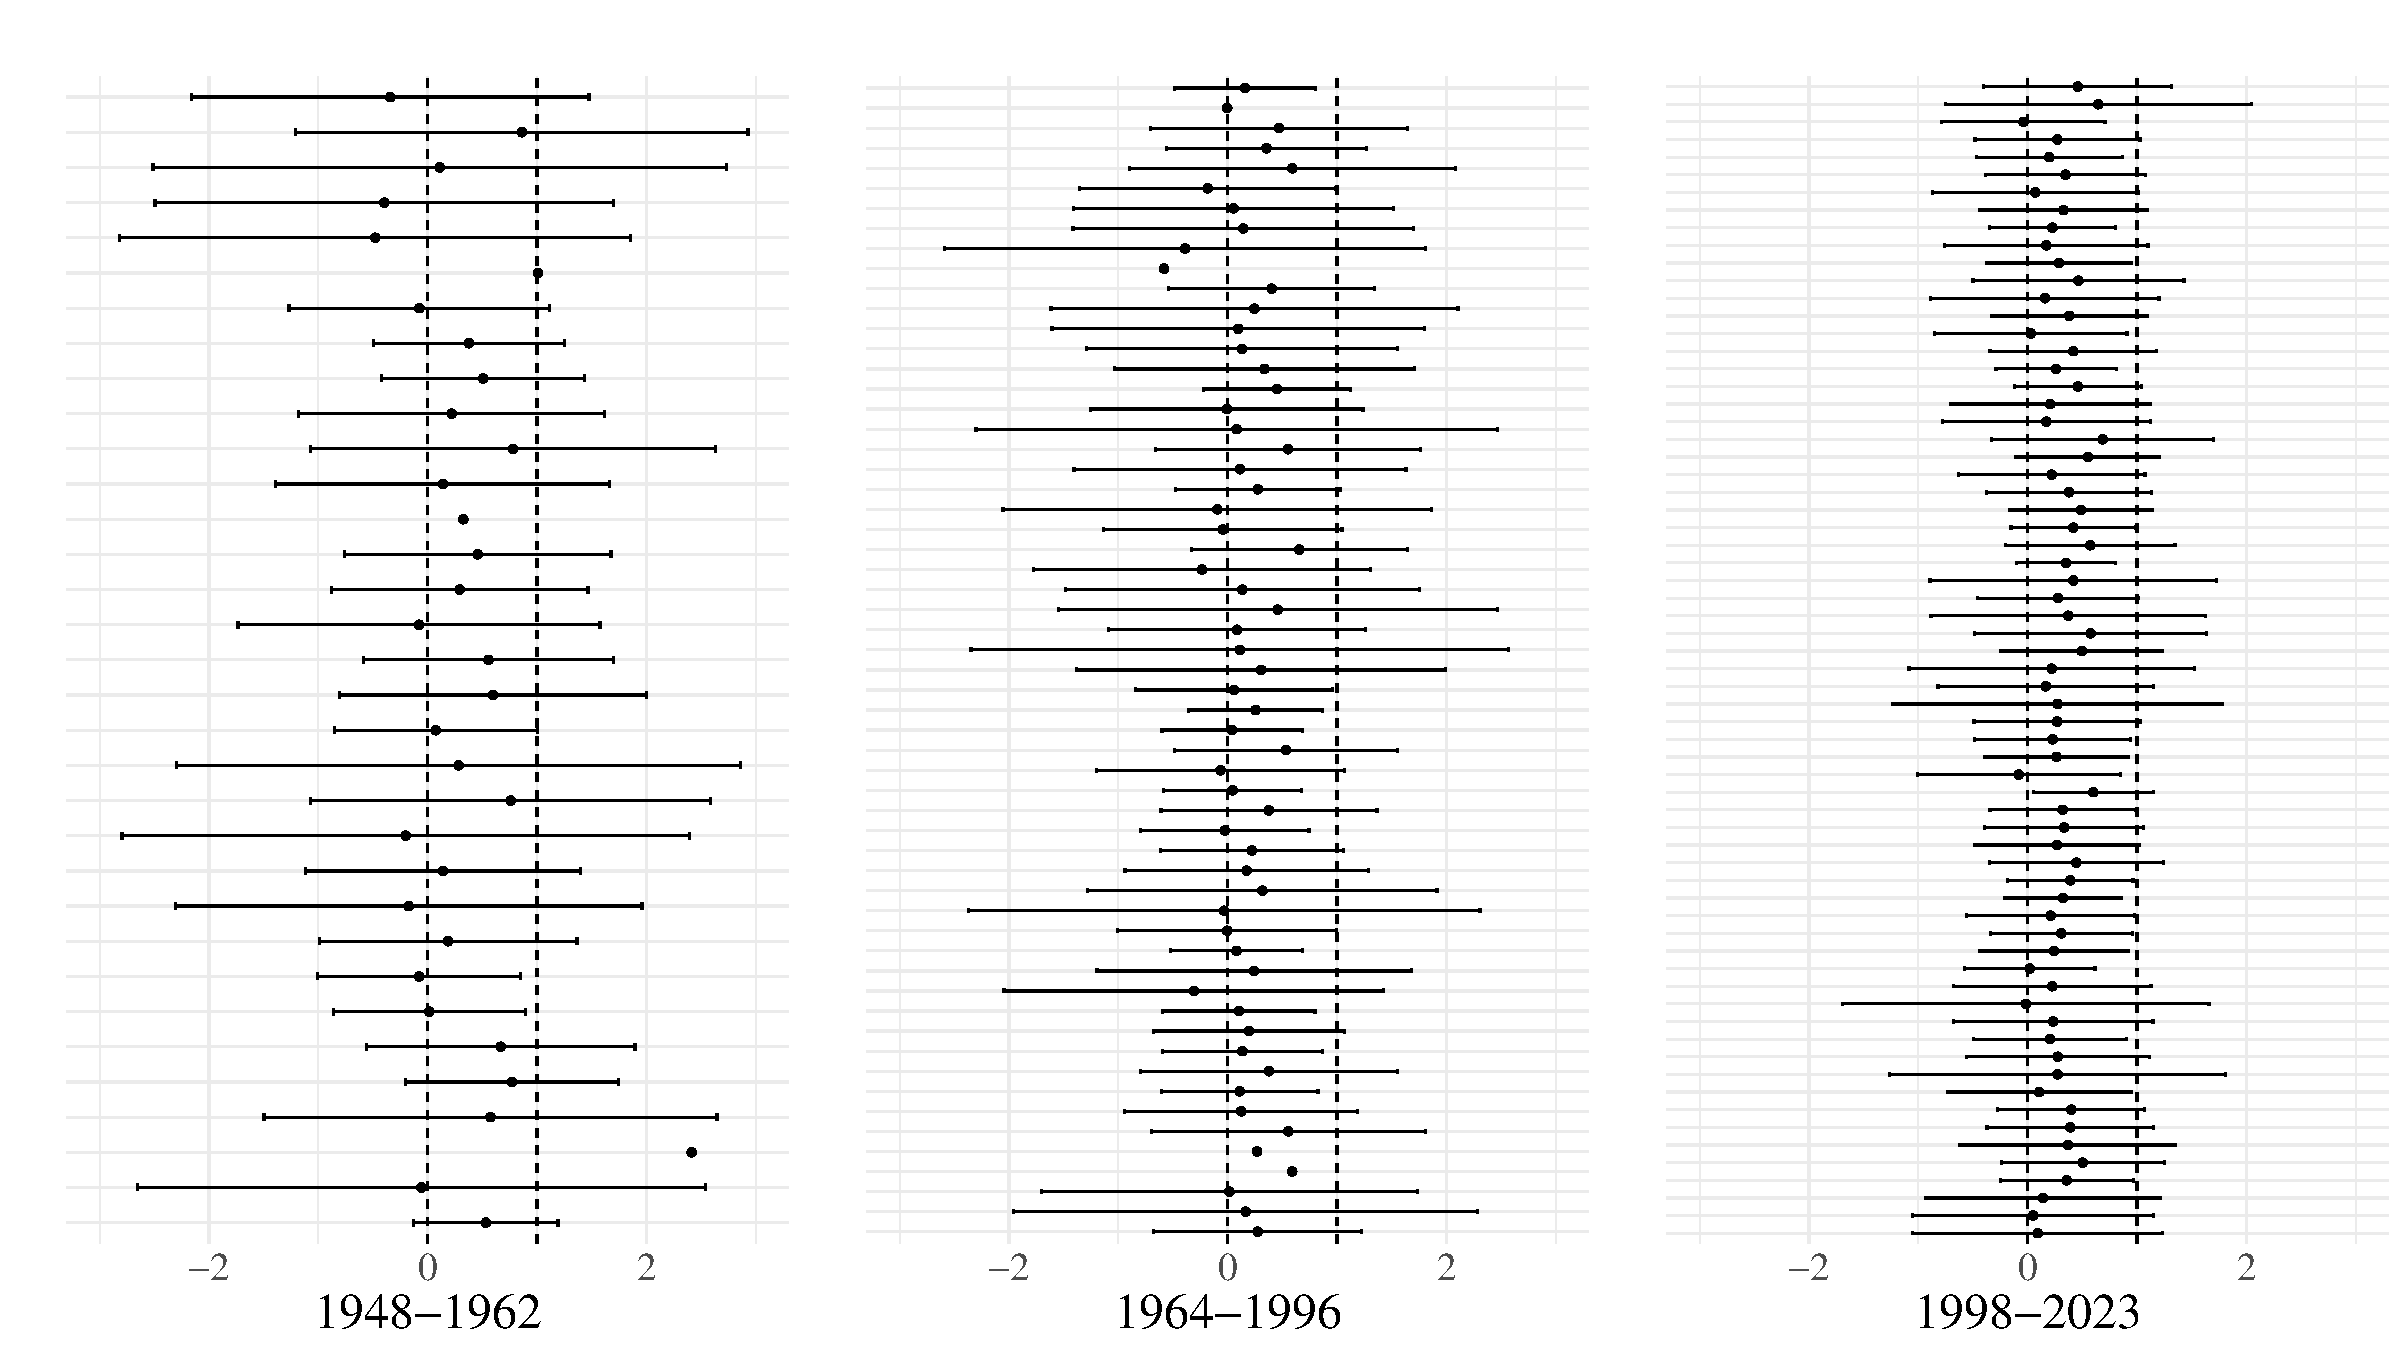
\includegraphics[width=.75\textwidth]{../figures/elasticity_est/elasticity_byCode_hist.pdf}
\caption{Mean and std. deviation of elasticities, by industry, extended sample}
\label{fig:theta_byCode_hist}
\end{figure}

\begin{figure}[!h]
\centering
\includegraphics[width=.75\textwidth]{../figures/elasticity_est/elasticity_byYear_hist.pdf}
\caption{Mean of elasticities, by year, extended sample}
\label{fig:theta_byYear_hist}
\end{figure}

\clearpage
% %%%%%%%%%%%%%%%%%%%%%%%%%%%%%%%%%%%%%%%%%%%%%%%%%%%%%%%%%%
% %%%%%%%%%%%%%%%%%%%%%%%%%%%%%%%%%%%%%%%%%%%%%%%%%%%%%%%%%%
% Bibliography
% %%%%%%%%%%%%%%%%%%%%%%%%%%%%%%%%%%%%%%%%%%%%%%%%%%%%%%%%%%
% %%%%%%%%%%%%%%%%%%%%%%%%%%%%%%%%%%%%%%%%%%%%%%%%%%%%%%%%%%

\bibliography{../../mylibrary.bib} 


\end{document}